\nonstopmode
\documentclass[10pt, a4paper]{article}
%\usepackage{subfig}

\parindent=20pt
\parskip=8pt
\usepackage[width=15.5cm, left=3cm, top=2.5cm, height= 24.5cm]{geometry}
\usepackage[spanish]{babel}
\usepackage[utf8]{inputenc}
\usepackage{fancyhdr}
\usepackage{multirow}
\usepackage{rotating}
\usepackage{indentfirst}
\usepackage{latexsym}
\usepackage{caratula}
\usepackage{gnuplottex}
\usepackage{epsfig}
\usepackage{lastpage}
\usepackage{amsfonts}
\usepackage{listings}
\usepackage[export]{adjustbox}
\usepackage{pdfpages}
\lstset{language=C}
\usepackage[ruled,vlined,linesnumbered]{algorithm2e}
\usepackage{graphicx}
\usepackage{float}
\usepackage{color}

\graphicspath{{imgs/}}



% Acomodo fancyhdr.
\pagestyle{fancy}
\thispagestyle{fancy}
\addtolength{\headheight}{1pt}
\lhead{Algoritmos y Estructuras de Datos III}
\rhead{TP2}
\cfoot{\thepage /\pageref{LastPage}}
\renewcommand{\footrulewidth}{0.4pt}
\renewcommand{\thesubsubsection}{\thesubsection.\alph{subsubsection}}




\author{Algoritmos y Estructuras de Datos III, DC, UBA.}
\date{}
\title{}

\begin{document}
	
\thispagestyle{empty}
\materia{Algoritmos y Estructuras de Datos III}
\submateria{Trabajo Pr\'actico N$^{\circ}$2}
\titulo{}
\integrante{Izcovich, Sabrina}{550/11}{sizcovich@gmail.com}
\integrante{Garcia Marset, Matias}{356/11}{matiasgarciamarset@gmail.com}
\integrante{Orellana, Ignacio}{229/11}{nacho@foxdev.com.ar}
\integrante{Vita, Sebastián}{149/11}{sebastian\_vita@yahoo.com.ar}

\maketitle

\tableofcontents
\newpage

\section{Introducci\'on}
Este trabajo práctico consiste en la resolución de ciertos problemas algorítmicos que cumplen con restricciones impuestas por la cátedra, como por ejemplo el orden de complejidad máximo de los mismos, entre otras. Para justificar las implementaciones de los problemas en cuestión, fue necesaria la utilización de herramientas lógico-matemáticas que serán mencionadas a lo largo del desarrollo de cada ejercicio.\newline
Para comprobar que nuestras soluciones resolvieran correctamente los problemas propuestos, debimos dividir el análisis de los mismos en secciones a fin de estudiar minuciosamente las características de éstos. Estas secciones se dividen de la siguiente forma:

\begin{itemize}
\item \textbf{Problema a resolver:} En esta sección, nos encargamos de describir detalladamente el problema a resolver dando ejemplos del mismo y sus soluciones.
\item \textbf{Resolución coloquial:} En esta parte, nos dedicamos a explicar de forma clara, sencilla, estructurada y concisa las ideas desarrolladas para la resolución del problema en cuestión. Para ello, decidimos utilizar pseudocódigo y lenguaje coloquial combinando ambas herramientas de manera adecuada.
\item \textbf{Demostración de correctitud:} Utilizamos este apartado para justificar que el punto anterior resuelve efectivamente el problema y demostramos formalmente la correctitud del mismo.
\item \textbf{Complejidad del algoritmo:} En esta sección, nos ocupamos de deducir una cota de complejidad temporal del algoritmo propuesto en función de los parámetros considerados como correctos. Por otro lado, justificamos por qué el algoritmo desarrollado para la resolución del problema cumple con la cota dada.
\item \textbf{Instancias posibles:} Este sector presenta un conjunto de instancias que permiten verificar la correctitud del programa implementado cubriendo todos los casos posibles y justificando la elección de los mismos. Dichas instancias fueron evaluadas por el algoritmo realizado y los resultados obtenidos fueron comprobados.
\item \textbf{Experimentación:} Por último, los tests consistieron en experimentaciones computacionales utilizadas para medir la performance del programa implementado. Para ello, debimos preparar un conjunto de casos de test que permitieran observar los tiempos de ejecución en función de los parámetros de entrada que fueran relevantes. Para ello, nos encargamos de generar instancias aleatorias como también particulares. Para que los resultados fueran visibles y claros, utilizamos una comparación gráfica entre los tiempos medidos y la complejidad teórica calculada.
\item \textbf{Código fuente:} En este apéndice, presentamos las funciones relevantes del código fuente que implementa la solución propuesta. Para ello, decidimos utilizar el lenguaje \verb*#C++# dado que éste cuenta con la librería $stl$ que proporciona las estructuras necesarias para la realización de dicha tarea.
\end{itemize}
\newpage

\section{Ejercicio 1}
\subsection{Problema a resolver}
El siguiente problema consiste en hallar un algoritmo capaz de dividir un conjunto de tareas ordenadas de forma tal que la realización de las mismas tenga costo total mínimo. El problema se ubica en una imprenta que cuenta con dos máquinas capaces de realizar distintas tareas de impresión. Estas máquinas deben ser preparadas de acuerdo al trabajo que vayan a realizar en ese momento. Dicha preparación requiere de un costo específico que depende del trabajo a realizar y del último ejecutado en esa máquina.\newline
\newline
Es importante considerar que los trabajos, $t_{1}$,...,$t_{n}$, pueden ser asignados a cualquiera de las dos máquinas, pero siempre respetando el orden en el que ingresan.\newline
\newline
Los datos otorgados consisten en los costos para preparar una máquina para el trabajo $t_{i}$ si antes se elaboró $t_{j}$, para cada par $t_{i}$ y $t_{j}$, con $j < i$. Por otro lado, se conoce el costo de preparar una máquina para cada trabajo al iniciar el día. Debe tenerse en cuenta que los costos son enteros positivos.\newline
\newline
El objetivo del problema consiste, entonces, en tomar la información de los trabajos a realizar y que el algoritmo generado sea capaz de indicar en qué máquina debe realizarse cada uno de ellos para que la suma de los costos de preparación de los mismos sea mínima.\newline
\newline
\textbf {Formatos de entrada y salida:}\newline
\newline
La entrada contiene varias instancias del problema. La primera línea de cada instancia contiene un entero positivo $n$ que indica la cantidad de trabajos ($t_{1},...,t_{n}$) a organizar. A esta línea le siguen $n$ líneas donde, en cada una de ellas, se indican los costos de preparación de cada trabajo. La $i$-ésima línea consta de los siguientes valores:

$$c_{0i}\ c_{1i}\ ...\ c_{(i-1)i}$$


donde \textbf{$c_{0i}$} es el costo de preparación de una máquina para $t_{i}$ si $t_{i}$ es el primer trabajo a realizar en esa máquina y $c_{ji}$ es el costo de preparación de una máquina para $t_{i}$ si $t_{j}$ es el último trabajo realizado en esa máquina. La entrada concluye con una línea comenzada por 0.\newline

La salida debe contener una línea por cada instancia de entrada, con el siguiente formato:

$$C\ k\ i_{1}\ ...\ i_{k}$$


donde \textbf{$C$} es el costo total de la solución, $k$ es la cantidad de trabajos asociados a una de las máquinas y los valores $i_{1},...,i_{k}$ son los índices de los trabajos asignados a esa máquina.\newline

En lo que sigue, presentaremos dos ejemplos del problema a resolver:
\begin{itemize}
\item {\large{\textbf{Ejemplo 1:}}}\newline
\newline
Para este ejemplo, decidimos elegir un posible caso del problema. En éste, pueden recorrerse los trabajos a realizar de forma ordenada hasta llegar a la solución óptima.\newline
\newline
\textbf{Formato de entrada:}
$$5$$
$$1$$
$$3\ \ 2$$
$$2\ \ 4\ \ 6$$
$$6\ \ 7\ \ 4\ \ 2$$
$$6\ \ 9\ \ 3\ \ 5\ \ 8$$

\begin{figure}[H] %[h] Aqui [b] para button [t] para top
\begin{center}
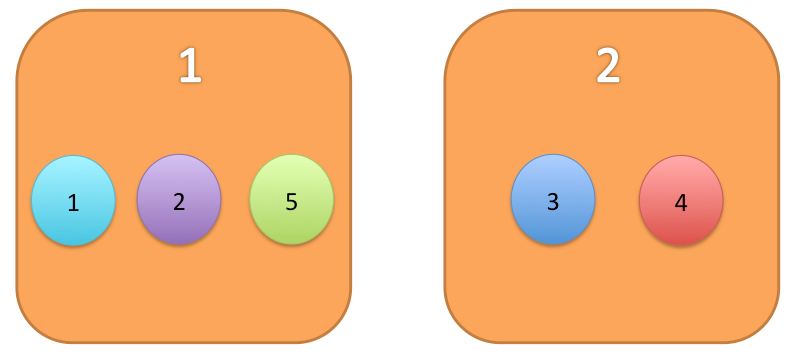
\includegraphics[width=250pt]{../imgs/ejemplo1ej1.jpg}
\caption{Ejemplo 1.}
\end{center}
\end{figure}

\textbf{Formato de salida:}
$$10\ \ 3\ \ 1\ \ 2\ \ 5$$
\item {\large{\textbf{Ejemplo 2:}}}\newline
\newline
En este caso, contrariamente al anterior, decidimos mostrar una situación en la que resultara extremadamente importante verificar todas las opciones posibles antes de tomar algún tipo de decisión sobre el armado de la solución al problema. En este caso, hasta no llegar al costo del último trabajo, cualquier decisión previa resulta inútil.\newline
\newline
\textbf{Formato de entrada:}
$$5$$
$$3$$
$$3\ \ 2$$
$$2\ \ 4\ \ 5$$
$$6\ \ 7\ \ 4\ \ 3$$
$$1\ \ 15\ \ 35\ \ 23\ \34$$

\begin{figure}[H] %[h] Aqui [b] para button [t] para top
\begin{center}
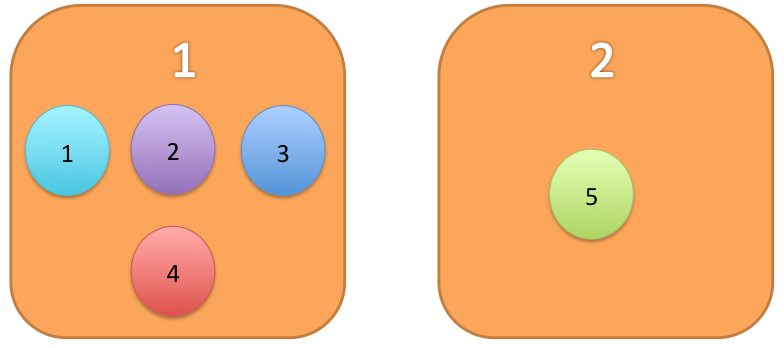
\includegraphics[width=250pt]{../imgs/ejemplo2ej1.jpg}
\caption{Ejemplo 2.}
\end{center}
\end{figure}

\textbf{Formato de salida:}
$$14\ \ 4\ \ 1\ \ 2\ \ 3\ \ 4$$
\end{itemize}

\subsection{Resolución coloquial}

Para resolver el problema descrito, consideramos armar todas las permutaciones posibles de los trabajos en las dos máquinas disponibles para realizarlos. Dado que contamos con dos máquinas y $n$ trabajos, las posibles combinaciones son $2^{n}$, siendo esta opción altamente costosa. Es entonces que decidimos resolver el problema utilizando $programación\ dinámica$.\newline
\newline
La $programación\ dinámica$, al igual que el método de Divide \& Conquer, resuelve problemas combinando las soluciones de sus subproblemas. A diferencia de este último, la $programación\ dinámica$ resuelve cada subproblema una única vez y almacena su solución en una tabla, evitando el trabajo de recomputar la respuesta cuando éste haya sido evaluado previamente.\newline
\newline
Luego, decidimos que nuestro programa almacenara las subsoluciones en una matriz del siguiente modo:
\begin{figure}[H]
\begin{center}
    \begin{tabular}{ l | l | l | l | l | l | l |}
    \multicolumn{7}{ |c| }{Máquina 1} \\
    \hline
    \multirow{5}{*}{\rotatebox{90}{\mbox{\centering{Máquina 2}}}} & \textbf{i/j} & \textbf{0} & \textbf{1} & ... & \textbf{(n-1)} & \textbf{n}\\ \cline{2-7}
    & \textbf{0} & $x_{00}$ & $x_{01}$ & ... & $x_{0(n-1)}$ & $x_{0n}$  \\ \cline{2-7}
   & \textbf{1} & $x_{10}$ & / & ... & $x_{1(n-1)}$ & $x_{1n}$ \\ \cline{2-7}
   & ... & ... & ... & ... & ... & ...\\ \cline{2-7}
   & \textbf{n} & $x_{n0}$ & $x_{n1}$ & ... & $x_{n(n-1)}$ & / \\ \cline{2-7}
    \end{tabular}
\caption{Matriz de almacenamiento de subproblemas calculados.}
\end{center}
\end{figure}
donde $x_{nm}$ representa el menor costo de realizar el trabajo $max(n,m)+1$ si la Máquina 1 realizó el trabajo $n$ y la 2 el $m$ previamente. Por otro lado, '/' representa que dicha casilla no puede ser completada dado que $i = j$, y un mismo trabajo no puede haberse realizado en ambas máquinas en una ejecución. El valor 0 representa el estado inicial de cada máquina.\newline
\newline
Por lo tanto, los casos que contempla nuestro algoritmo son de la siguiente forma:
\begin{figure}[H] %[h] Aqui [b] para button [t] para top
\begin{center}
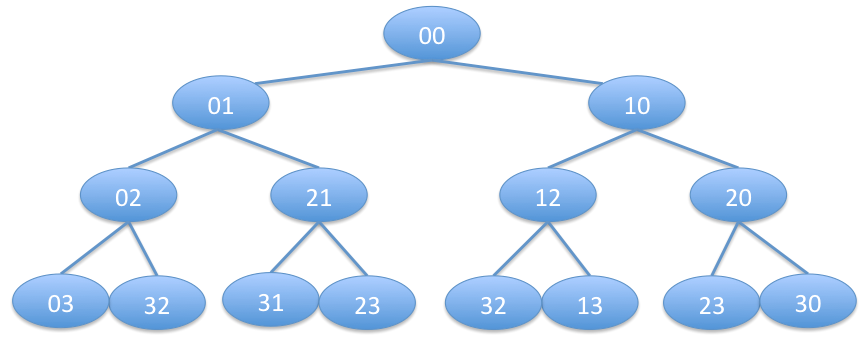
\includegraphics[width=400pt]{../imgs/arbol.jpg}
\caption{Árbol de decisiones del modelado del problema.}{\textit{Prueba con cantidad de trabajos = 3.}}
\end{center}
\end{figure}
Donde en cada \raisebox{-.1\height}{
\includegraphics[width=40pt]{../imgs/leyendaArbol.jpg}}, $m$ representa al último trabajo realizado en la máquina 1 y $n$ al realizado en la máquina 2. El estado \raisebox{-.1\height}{
\includegraphics[width=40pt]{../imgs/Cerocero.jpg}} representa el estado inicial del problema, en el que no hay trabajos. Como puede observarse, se repiten una gran cantidad de casos dado que las máquinas son indistinguibles entre sí, luego \raisebox{-.1\height}{
\includegraphics[width=40pt]{../imgs/ij.jpg}}=\raisebox{-.1\height}{
\includegraphics[width=40pt]{../imgs/ji.jpg}} para cada $i \neq j$. Por lo tanto, recalcular los costos resulta, además de altamente costoso, innecesario, siendo la $programación\ dinámica$ un método adecuado para la realización del algoritmo.

El pseudocódigo que resuelve el problema es el siguiente:\newline
\newline
%no se hacer pseudo sobre matrices jijiji
\begin{algorithm}[H]
    \SetAlgoLined
    \caption{MinimizacióndeCostosdeTareas}
    \KwIn{Entero $m1$, Entero $m2$, Entero $cantidadDeTrabajos$, Costos $cs$, Matriz $valores$}
    \KwOut{Costo $c$}
    
    Entero $siguienteTrabajo$ = $max(m1,m2)+1$\\ 
    \If{$siguienteTrabajo > cantidadDeTrabajos$}{
        $c$ = 0
    }\\
    \eIf{$valores[m1][m2]>-1$}{
        $c$ = $valores[m1][m2]$
    }{
        Entero $costo1$ = cs[siguienteTrabajo-1][m1] +\\ MinimizacióndeCostosdeTareas(siguienteTrabajo,m2)\\
        Entero $costo2$ = cs[siguienteTrabajo-1][m2] +\\ MinimizacióndeCostosdeTareas(m1, siguienteTrabajo)\\
        \eIf{$costo1 < costo2$}{
            $valores[m1][m2] = costo1$\\
            $valores[m2][m1] = costo1$\\        
            $c$ = $costo1$\\
        }{
            $valores[m1][m2] = costo2$\\
            $valores[m2][m1] = costo2$\\        
            $c$ = $costo2$\\
        }
    }\\
    \textbf{devolver} $c$
\end{algorithm}

\begin{algorithm}[H]
    \SetAlgoLined
    \caption{inicializarMinimizacionDeCostos}
    \KwIn{Entero $cantidadDeTrabajos$}
    \KwOut{Costo $c$, Entero $cantidadAsociada$, $listaIndices$}



    \lIf{$cs = \emptyset$}{\textbf{devolver} 0, 0, $ListaVacia$}\\
    Entero $costoMinimo$ = MinimizacióndeCostosdeTareas(0,0)\\

    Lista $maquina1$\\

    \For{Entero i=1 a $cantidadDeTrabajos$}{
        \eIf{$valores[i][m2] < valores[m1][i]$}{
            $m1 = i$\\
        }{
            $m2 = i$\\
            $maquina1$ \leftarrow i\\
        }
    }

    \textbf{devolver} $costoMinimo, |maquina1|, maquina1$\\

    
\end{algorithm} 

Donde $Costos$ es una matriz que contiene los costos de poner un trabajo $i$ en una máquina si previamente se realizó el trabajo $j$ en ella misma, con $j<i$. Por otro lado, $maquina1$ consiste en una lista de los trabajos que realiza la máquina a la que se le inserta el primer trabajo.

\newpage
\subsection{Demostración de correctitud}

Veamos que el algoritmo realizado es correcto. Empecemos por demostrar que cada subproblema es óptimo. Para ello, consideremos que cada uno de éstos consiste en determinar en qué máquina debe ubicarse el trabajo $x$ si en la 1 se encuentra el $i$ y en la 2 el $j$, con $x=max(i,j)+1$, tal que el costo sea mínimo. Esto significa que, dadas dos opciones posibles, nuestro algoritmo calcula ambas y selecciona la de menor costo en cada subproblema. De este modo, nuestro algoritmo recorre todas las secuencias de decisiones almacenando las subsoluciones óptimas.

Luego, demostremos que nuestro algoritmo cumple con el Principio de optimalidad de Bellman para corroborar su correctitud.\footnote{Dada una secuencia óptima de decisiones, toda subsecuencia de ella es, a su vez, óptima.} Para ello, supongamos que éste devuelve la solución óptima $S$. Dicha solución se encuentra conformada por todas subsoluciones óptimas salvo una, $x_{i}$. Luego, reemplacemos $x_{i}$ por la solución óptima de su subproblema correspondiente\footnote{Sabemos que existe una subsolución óptima pues estamos ante un conjunto no vacío de soluciones y todo conjunto acotado no vacío alcanza un mínimo local.}, llamemos $S^*$ a esta nueva solución. Pero entonces, $S^*$ tiene un costo final menor que $S$. Esto resulta absurdo pues supusimos que $S$ era solución óptima. Luego, todas las subsoluciones de $S$ son óptimas implicando que la solución final también lo es. Entonces, queda demostrado que nuestro algoritmo cumple con el Principio de optimalidad de Bellman confirmando su optimalidad.

% demostrar usando http://webdiis.unizar.es/asignaturas/EDA/ea/slides/4-Programacion%20dinamica.pdf
\subsection{Complejidad del algoritmo}

Veamos que nuestro agoritmo cumple con la complejidad requerida. Para ello, llamemos $n$ a la cantidad total de trabajos a realizar:
\begin{itemize}
\item En primer lugar, la función \textbf{inicializarMinimizacionDeCostos} inicializa la matriz $valores$ con una dimensión de $n^*n$ y aplica una única vez la función \textbf{resize} ($\mathcal{O}(n)$)\footnote{http://en.cppreference.com/w/cpp/container/vector/resize}. Dicha matriz se encuentra representada por un vector de vectores cuyo espacio de memoria es reservado para que las asignaciones se realicen en $\mathcal{O}(1)$. Dado que la función la recorre una única vez para inicializarla, el costo temporal resulta $\mathcal{O}(n^{2})$. Por otro lado, se utilizan las funciones $size()$($\mathcal{O}(1)$)\footnote{http://en.cppreference.com/w/cpp/container/vector/size} y $push\_back()$($\mathcal{O}(1)$)\footnote{http://en.cppreference.com/w/cpp/container/vector/push\_back} pero, dado que sus complejidades no resultan significativas frente a la complejidad final de la función, no son consideradas para el cálculo de la misma. Luego, la complejidad de \textbf{inicializarMinimizacionDeCostos} resulta $\mathcal{O}(n^{2})$.

\item Por otro lado, se realiza un llamado a \textbf{MinimizacióndeCostosdeTareas}. Veamos que una vez completada la matriz $valores$, la complejidad de la función recursiva se torna constante y puede verse acotada por el tamaño de la matriz ($n^{2}$).
\begin{itemize}
\item En cada llamada recursiva a \textbf{MinimizacióndeCostosdeTareas}, se determina en qué máquina se ubica el $sigTrabajo$. Para tomar dicha decisión, se realizan operaciones de tiempo lineal y se ejecuta recursivamente la función dos veces. En la primera, agregando el trabajo en la máquina 1 y, en la segunda, agregando el trabajo en la máquina 2. De esta manera, se calculan las soluciones a dichos subproblemas a menos que los resultados de éstos ya se encuentren en la matriz $valores$ (dado que ésta abarca todas las subsoluciones posibles), acotando dicha ejecución por $\mathcal{O}(n^{2})$. A partir de esto, podemos determinar que el peor caso consiste en llenar la matriz entera ($\mathcal{O}(n^{2})$) y que las soluciones a las llamadas recursivas siguientes se encuentren en ella, tornándolas constantes. Por lo tanto, el costo temporal de la llamada recursiva se encuentra acotado por la matriz, luego, por $\mathcal{O}(n^{2})$. 

\item Una vez almacenadas todas las subsoluciones en $valores$, se procede armando la solución final. Para ello, se reproducen las decisiones tomadas en cada paso a partir de la matriz. Dicho procedimiento se ejecuta en \textbf{inicializarMinimizacionDeCostos}, con un ciclo de 1 hasta $n$ que compara, en cada paso, dos valores enteros de la matriz. Luego, este extracto tiene una complejidad de $\mathcal{O}(n)$ ya que las comparaciones se realizan en $\mathcal{O}(1)$.

\end{itemize}
\item Por lo tanto, el costo temporal de \textbf{inicializarMinimizacionDeCostos} es $\mathcal{O}(n^{2})$ y el de \textbf{MinimizaciondeCostosdeTareas} es $\mathcal{O}(n^{2})$ y, dado que dichas funciones se realizan en forma paralela, la complejidad temporal final es $\mathcal{O}(2n^{2})$, que se encuentra acotado por $\mathcal{O}(n^{2})$. 
\end{itemize}

\subsection{Instancias posibles}
Para verificar la correctitud de nuestro programa, dispusimos variar estratégicamente las instancias de entrada al ejecutarlo.
\begin{itemize}
\item En primer lugar, ejecutamos el programa ingresando trabajos de igual costo independientemente del trabajo realizado anteriormente. De este modo, verificamos que nuestro algoritmo organizara los trabajos tal como esperado cuando más de una combinación posible fuera solución.\newline

\textbf{Parámetro de entrada:} $$5$$
$$5$$
$$5\ \ 5$$
$$5\ \ 5\ \ 5$$
$$5\ \ 5\ \ 5\ \ 5$$
$$5\ \ 5\ \ 5\ \ 5\ \ 5$$
\textbf{Parámetro de salida:} $$25\ \ 4\ \ 1\ \ 2\ \ 3\ \ 4$$\\
\item Por otra parte, probamos no ingresar ningún trabajo para corroborar que la salida estuviera comprendida por un costo 0, una cantidad de trabajos asociados a una máquina igual a 0 y una lista vacía.\newline

\textbf{Parámetro de entrada:} $$0$$
\textbf{Parámetro de salida:} $$0\ \ 0 \ \ 0$$

\item Luego, probamos ingresar costos que implicaran que todos los trabajos debían realizarse en una misma máquina con el fin de verificar que esto, efectivamente, ocurriera.\newline

\textbf{Parámetro de entrada:} $$5$$
$$4$$
$$7\ \ 4$$
$$8\ \ 9\ \ 5$$
$$6\ \ 7\ \ 5\ \ 2$$
$$5\ \ 6\ \ 8\ \ 9\ \ 1$$
\textbf{Parámetro de salida:} $$16\ \ 5 \ \ 1\ \ 2\ \ 3\ \ 4\ \ 5$$
\end{itemize}

De este modo, logramos abarcar los casos límite en los que la implementación pudiera haber encontrado algún problema. Dado que los resultados obtenidos fueron los esperados, determinamos que para todas las instancias válidas posibles de entrada nuestra implementación resulta correcta.

\subsection{Experimentación}
Para las pruebas de complejidad empírica, generamos instancias aleatorias de costos de los trabajos alterando la cantidad de los mismos. Estas instancias fueron generadas en $C++$ con la función $rand()$. La cantidad de trabajos generados se comprendió entre 100 y 32300, agregando de a 100 en cada iteración. Las mediciones de tiempo en nanosegundos se realizaron con la función $high\ resolution\ clock$\footnote{http://en.cppreference.com/w/cpp/chrono/high\_resolution\_clock} de la librería $Chrono$ de $C++$. Debido a que éstas fueron realizadas en nanosegundos, las pruebas cuyo tamaño de entrada era menor a 1000 se realizaban en mayor tiempo que las instancias más grandes pues el procesador les otorgaba menos atención al realizar cambio de contexto. De este modo, logramos medir las pruebas de nuestro algoritmo para comprobar que la complejidad correspondiera con la mencionada anteriormente.

Las funciones de complejidad con las que se compararon nuestros gráficos de tiempo fueron ajustadas por algoritmos matemáticos (proporcionados por \textbf{sci davis}). Dichos algoritmos se encargaron de multiplicarle y sumarle constantes a las funciones con el fin de que éstas se ajustaran a nuestros resultados sin modificar el comportamiento de las funciones utilizadas para comparar.

\begin{figure}[H] %[h] Aqui [b] para button [t] para top
\begin{center}
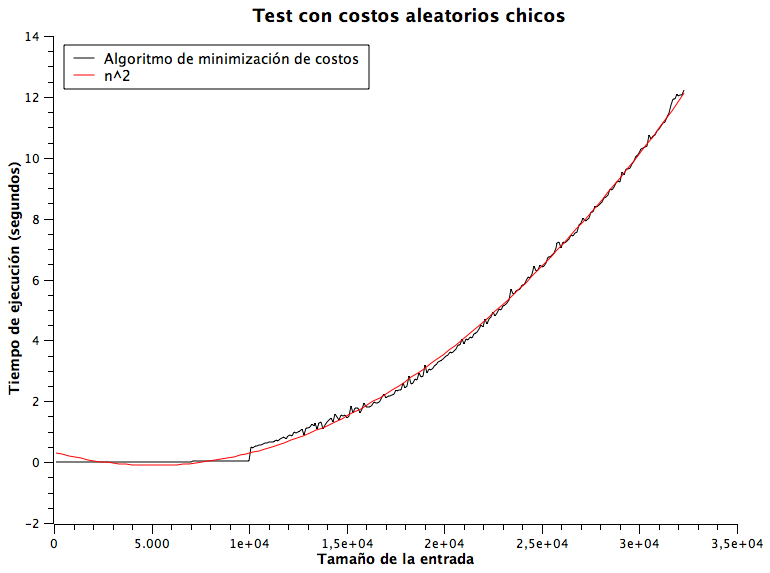
\includegraphics[width=350pt]{../tests/ej1/testChico.png}
\end{center}
\end{figure}
En este caso, utilizamos instancias de números aleatorios entre 1 y 150. En este gráfico, se puede ver de forma clara que la función de la complejidad se adapta perfectamente a los datos obtenidos. De este modo, se deja en evidencia la complejidad esperada.


La función utilizada para aproximar nuestros valores resultantes luego de las distintas ejecuciones fue $a_{0} + a_{1}x + a_{2}x^{2}$.
En este caso, los valores que aproximan la función a nuestros datos son:
$$desde\ x = 100\ a\ x = 32.300$$
$$a_{0} = 0,32423419158503$$
$$a_{1} = -0,00016812837387441$$
$$a_{2} = 1,65040451628269e^{-8}$$

% ---------------------------------------------------------------------------------------
% Polynomial fit of dataset: Table1_2, using function: a0+a1*x+a2*x^2
% Y standard errors: Unknown
% From x = 100 to x = 32.300
% a0  = 0,32423419158503 +/- 0,0215946299831477
% a1  = -0,00016812837387441 +/- 3,07784412487107e-06
% a2  = 1,65040451628269e-08 +/- 9,19965264096027e-11
% --------------------------------------------------------------------------------------
% Chi^2/doF = 0,0165295926762495
% R^2 = 0,998773136476792
% ---------------------------------------------------------------------------------------

\begin{figure}[H] %[h] Aqui [b] para button [t] para top
\begin{center}
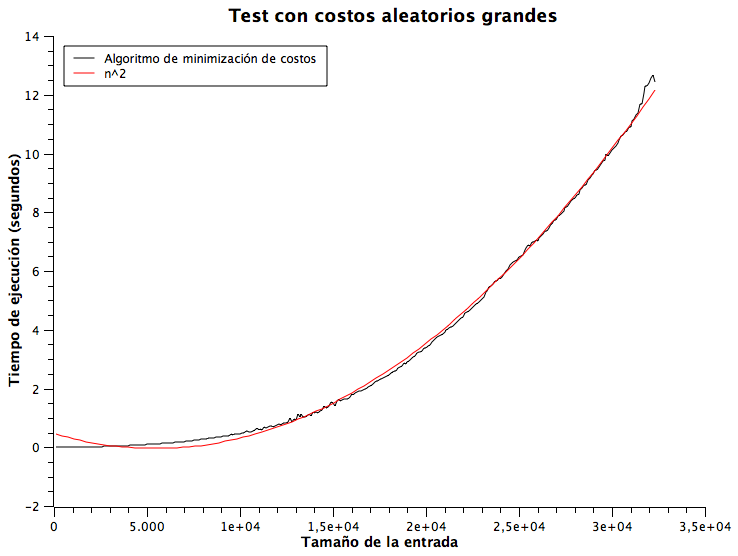
\includegraphics[width=350pt]{../tests/ej1/testGrande.png}
\end{center}
\end{figure}

En este caso, utilizamos instancias de números aleatorios entre 500 y 1500. Al igual que en la situación anterior, se puede observar que la función de complejidad se acerca perfectamente a los valores devueltos por las distintas ejecuciones del programa. En esta situación, encontramos que la magnitud de los costos de los trabajos no afectan la complejidad, y esto tiene sentido ya que la complejidad se encuentra determinada por la cantidad de trabajos ingresados.

La función utilizada para aproximar nuestros valores resultantes luego de las distintas ejecuciones fue $a_{0} + a_{1}x + a_{2}x^{2}$.
En este caso, los valores que aproximan la función a nuestros datos son:

$$desde\ x = 100\ a\ x = 32.300$$
$$a_{0}  = 0,463420767939423$$
$$a_{1}  = -0,000185064576979962$$
$$a_{2}  = 1,69442722903951e^{-8}$$

% ---------------------------------------------------------------------------------------
% [29/09/13 15:11 Plot: ''Graph1'']
% Polynomial fit of dataset: Table1_2, using function: a0+a1*x+a2*x^2
% Y standard errors: Unknown
% From x = 100 to x = 32.300
% a0  = 0,463420767939423 +/- 0,0259887707740958
% a1  = -0,000185064576979962 +/- 3,70188804599674e-06
% a2  = 1,69442722903951e-08 +/- 1,10661696857655e-10
% --------------------------------------------------------------------------------------
% Chi^2/doF = 0,0239117967063003
% R^2 = 0,998216395272766
% ---------------------------------------------------------------------------------------

\begin{figure}[H] %[h] Aqui [b] para button [t] para top
\begin{center}
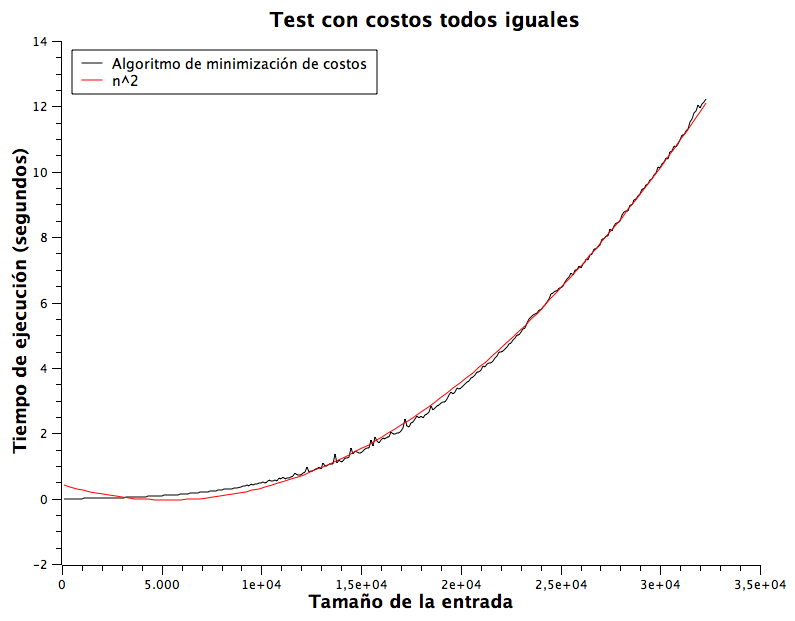
\includegraphics[width=350pt]{../tests/ej1/testIguales.png}
\end{center}
\end{figure}

En este caso, utilizamos instancias cuyos valores son todos iguales. Esto implica que existen múltiples soluciones al problema, y que el programa debe contemplar cada una de ellas. Al observar los resultados, llegamos a la conclusión de que la cantidad de soluciones posibles no es un factor significante a la hora de medir la complejidad de las ejecuciones. Esto se debe a que, a pesar de encontrar una solución al problema, el algoritmo debe probar con todas las demás posibilidades para comprobar que no exista una mejor.

La función utilizada para aproximar nuestros valores resultantes luego de las distintas ejecuciones fue $a_{0} + a_{1}x + a_{2}x^{2}$.
En este caso, los valores que aproximan la función a nuestros datos son:

$$desde\ x = 100\ a\ x = 32.300$$
$$a_{0}  = 0,424466923410826$$
$$a_{1}  = -0,000176224064649403$$
$$a_{2}  = 1,66520770037108e^{-8}$$


% ---------------------------------------------------------------------------------------
% [29/09/13 15:27 Plot: ''Graph1'']
% Polynomial fit of dataset: Table1_2, using function: a0+a1*x+a2*x^2
% Y standard errors: Unknown
% From x = 100 to x = 32.300
% a0  = 0,424466923410826 +/- 0,0221964720229293
% a1  = -0,000176224064649403 +/- 3,16061236730305e-06
% a2  = 1,66520770037108e-08 +/- 9,44987080940012e-11
% --------------------------------------------------------------------------------------
% Chi^2/doF = 0,0174278400512325
% R^2 = 0,998690483561816
% ---------------------------------------------------------------------------------------



\newpage

\section{Ejercicio 2}
\subsection{Problema a resolver}
Este problema radica en una organización encargada de replicar contenido para su red de entrega de información en Internet. Para esto, dispone de $n$ servidores interconectados mediante $m$ enlaces $backbone$ de alta velocidad. El servidor $máster$ es el primero en recibir los nuevos datos a replicar y es el encargado de transmitir dicha información a otros servidores. Éstos guardarán su propia copia y la retransmitirán hasta que todos los servidores contengan la nueva información. Es importante considerar que todos los enlaces transmiten la misma información, que los $n$ servidores se encuentran interconectados por dichas conexiones y que los enlaces $backbone$ tienen costo en función del tráfico que transmiten.

La organización seleccionó dos consultoras con el fin de resolver los siguientes problemas:
\begin{itemize}
\item El primero se basa en hallar un algoritmo capaz de encontrar el camino mínimo entre un conjunto de servidores. En el contexto del problema, esto consiste en elegir los enlaces que permitan distribuir la información a todos los servidores con un costo mínimo.

\item El segundo consiste en encontrar el servidor $máster$ de forma tal que la replicación de la información, que empieza una vez que el $máster$ recibe la información y termina cuando todos los servidores tienen su copia, se realice en el mínimo tiempo posible. Para ello, se considera que la información tarda el mismo tiempo en atravesar cualquier enlace y que cada servidor transmite simultáneamente a todos los vecinos elegidos.
\end{itemize}
\textbf {Formatos de entrada y salida:}\newline
\newline
La entrada contiene varias instancias del problema. La primera línea de cada instancia contiene un entero positivo $n$ que indica la cantidad de servidores (numerados de 1 a $n$), un espacio, y un entero no negativo $m$ que corresponde a la cantidad de enlaces. A esta línea le siguen $m$ líneas con la descripción de cada enlace (números separados por un espacio):

$$a_{j}\ b_{j}\ ...\ c_{j}$$


donde \textbf{$a_{j}$} y \textbf{$b_{j}$} son los servidores que el enlace $j$ conecta y \textbf{$c_{j}$} es el costo de usar el enlace $j$ (entero no negativo). La entrada concluye con una línea comenzada por 0.\newline

La salida debe contener una línea por cada instancia de entrada, con el siguiente formato:

$$C\ U\ k\ e_{1}^1\ e_{2}^1\ e_{1}^2\ e_{2}^2\...\ e_{1}^k\ e_{2}^k$$


donde \textbf{$C$} es el costo total de la solución, $U$ es el servidor elegido como $máster$, $k$ es la cantidad de enlaces y $e_{1}^i$ y $e_{2}^i$ son los extremos del $i$-ésimo enlace de la solución obtenida, para $i\ \in$ [1,$k$].\newline

En lo que sigue, presentaremos dos ejemplos del problema a resolver:
\begin{itemize}
\item {\large{\textbf{Ejemplo 1:}}}\newline
\newline
El siguiente ejemplo consiste en un caso simple de la situación a resolver con la particularidad de que existe más de una solución posible al problema. Como puede observarse, tanto el enlace (1,5) como el (5,4) forman parte de la solución óptima, pero de éstos se elige únicamente uno.\newline
\newline
\textbf{Formato de entrada:}
$$5\ 6$$
$$1\ \ 2\ \ 2$$
$$1\ \ 3\ \ 1$$
$$1\ \ 5\ \ 2$$
$$2\ \ 3\ \ 1$$
$$3\ \ 4\ \ 1$$
$$4\ \ 5\ \ 2$$

\begin{figure}[H] %[h] Aqui [b] para button [t] para top
\begin{center}
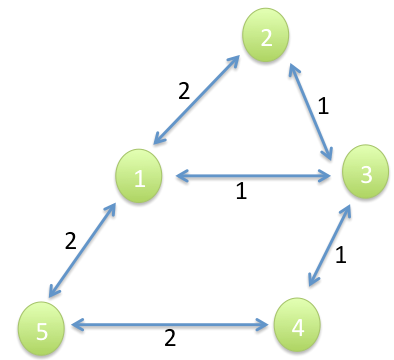
\includegraphics[width=210pt]{../imgs/ejemplo1ej2ent.jpg}
\caption{Ejemplo 1 - entrada.}
\end{center}
\end{figure}

\textbf{Formato de salida:}
$$5\ \ 2\ \ 4\ \ 1\ \ 2\ \ 1\ \ 5\ \ 2\ \ 3\ \ 3\ \ 4$$

\begin{figure}[H] %[h] Aqui [b] para button [t] para top
\begin{center}
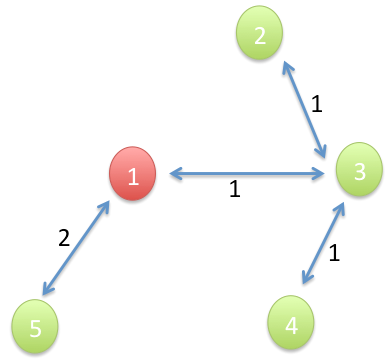
\includegraphics[width=210pt]{../imgs/ejemplo1ej2sal.jpg}
\caption{Ejemplo 1 - salida.}
\end{center}
\end{figure}
\item {\large{\textbf{Ejemplo 2:}}}\newline
\newline
Este ejemplo consiste en un caso usual de la situación planteada en el que puede verse de forma simple y clara la elección que debe realizar el algoritmo para hallar la solución óptima.\newline
\newline
\textbf{Formato de entrada:}
$$5\ 6$$
$$1\ \ 2\ \ 2$$
$$1\ \ 3\ \ 3$$
$$2\ \ 3\ \ 1$$
$$3\ \ 4\ \ 2$$
$$3\ \ 5\ \ 2$$
$$4\ \ 5\ \ 1$$

\begin{figure}[H] %[h] Aqui [b] para button [t] para top
\begin{center}
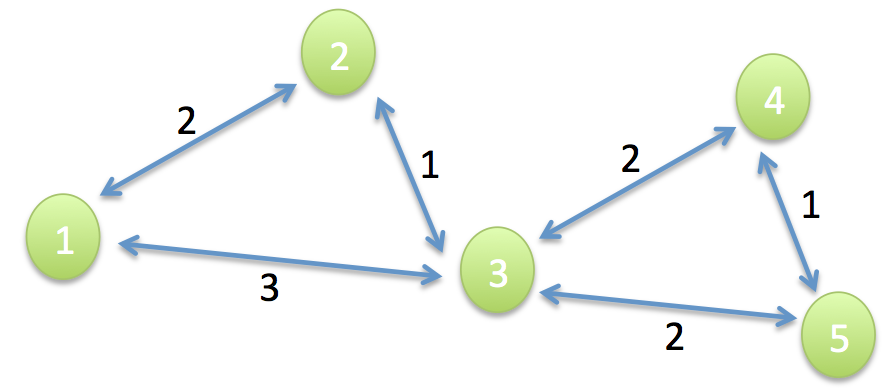
\includegraphics[width=300pt]{../imgs/ejemplo2ej2ent.jpg}
\caption{Ejemplo 2 - entrada.}
\end{center}
\end{figure}

\textbf{Formato de salida:}
$$8\ \ 3\ \ 4\ \ 1\ \ 3\ \ 2\ \ 3\ \ 3\ \ 4\ \ 3\ \ 5$$

\begin{figure}[H] %[h] Aqui [b] para button [t] para top
\begin{center}
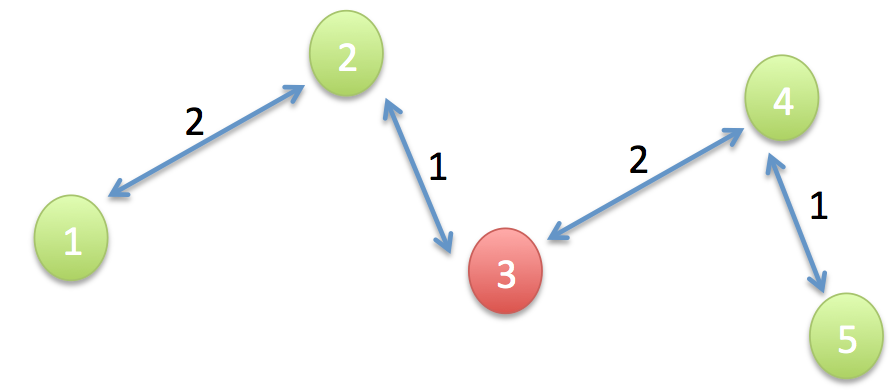
\includegraphics[width=300pt]{../imgs/ejemplo2ej2sal.jpg}
\caption{Ejemplo 2 - salida.}
\end{center}
\end{figure}

\subsection{Minimización de enlaces}
\subsubsection{Resolución coloquial}

 El problema planteado consiste en conectar todos los servidores de la red de forma tal que el costo de transmisión de datos sea el mínimo. Para poder resolver esto, decidimos utilizar un algoritmo que encontrara un Árbol Generador Mínimo\footnote{El peso de un árbol generador es la suma de los pesos de las aristas del árbol. Un árbol generador mínimo es uno con peso mínimo.} que contuviera los enlaces de menor peso necesarios para unir a todos los servidores. Para ello, utilizamos el algoritmo de $Kruskal$. Éste genera un conjunto de árboles que representan los nodos del grafo original. El algoritmo toma la menor arista (según su peso) y evalúa si sus extremos pertenecen a árboles distintos. En caso de así serlo, los une y agrega la arista al árbol generador mínimo. Si, por el contrario, los extremos forman parte del mismo árbol, el algoritmo descarta dicha arista.\newline
\newline
El pseudocódigo del algoritmo mencionado es el siguiente: \newline
\newline

\begin{algorithm}[H]
	\SetAlgoLined
	\caption{kruskal}
	\KwIn{Entero $CantidadServidores$, Grafo $G$}
	\KwOut{Grafo $Gr$}
    
    $//G = (V,E)$ \\
    ordenarDeMenorAMayorPorPeso $E$\\  
    \\ 
    Grafo $Gr \leftarrow$ $<>$\\
	\ForAll{$E$}{
        Entero $nodoA \leftarrow$ PrimerVertice $E$\\
        Entero $nodoB \leftarrow$ SegundoVertice $E$\\
        \If{find(nodoA) != find(nodoB)}{\\
            union(find($nodoA$), find($nodoB$)) \\
            Marcar($E$)
        }
	}\\
    \ForAll{$E$}{
        \If{EstaMarcado?($E$)}{\\
            Insertar($Gr$,$E$)   \\
        }
	}

	\textbf{devolver} $Gr$
\end{algorithm}

\newline
Para lograr que el algoritmo de Kruskal fuera más eficiente, decidimos aplicarle una mejora tanto a la función union como a la función find.\newline
\newline
En el caso de la función $find$, decidimos aplicar el método de $compresión\ de\ caminos$ que, al momento de retornar la raíz en la recursión, actualiza el padre de cada vértice visitado. Luego, cada nodo ya visitado tiene como padre a la raíz.\newline
\newline
Para la función $union$, implementamos el método $unión\ por\ rango$. Éste une el árbol de menor rango con la raíz del de mayor rango. Luego, la altura resultante es igual a la mayor de los dos. Si no se aplicara dicha función, la altura resultante sería la del árbol más grande +1 dado que éste se colocaría como hijo de la raíz del de menor tamaño. \newline
\newline
Los pseudocódigos de dichos algoritmos son los que se presentan a continuación:\newline
\newline
\begin{algorithm}[H]
	\SetAlgoLined
	\caption{find}
	\KwIn{Entero $nodo$, vector$<$Entero$>$ $padre$}
	\KwOut{Entero res}
	\If{nodo = Raiz(nodo)}{\textbf{devolver} $nodo$}
    
	\textbf{devolver} $Raiz(nodo) \leftarrow$ find(Raiz($nodo)$)
\end{algorithm}

\begin{algorithm}[H]
	\SetAlgoLined
	\caption{union}
	\KwIn{Entero $nodoA$, Entero $nodoB$, vector$<$Entero$>$ $padre$}
	\KwOut{Entero res}
	\eIf{AlturaDeLaComponente $nodoA$ $>$ AlturaDeLaComponente $nodoB$}{Raiz($nodoB$) = $nodoA$}{
    Raiz($nodoA$) = $nodoB$\\
    AlturaDeLaComponente $nodoB$++}
\end{algorithm}

Donde la función $Raiz(x)$ devuelve la raíz del árbol conteniendo el nodo $x$ y la función $AlturaDeLaComponente(x)$ devuelve la altura del árbol que comprende a $x$.

\subsubsection{Demostración de correctitud}

Para demostrar la correctitud de nuestro algoritmo, debemos probar que se cumplen las siguientes propiedades:
\begin{itemize}
\item Se unen todos los servidores mediante enlaces $backbone$.
\item La solución es óptima, es decir, no existe otra combinación de enlaces que una a todos los servidores y cuyo costo sea menor.
\end{itemize}

\newline

\textbf{Se unen todos los servidores mediante enlaces backbone:} \newline
\newline
La entrada de nuestro algoritmo es un grafo conexo. Esto significa que, para cualquier par de vértices ($v_{1}$, $v_{2}$) del grafo, existe al menos un camino que los une. \newline  
\newline
Sea $G$ el grafo de entrada de $n$ nodos y $m$ aristas, y $G'$ uno conformado por $n$ componentes conexas, donde cada una de ellas es un vértice de $G$.
En primer lugar, nuestro algoritmo comprueba si la inserción de cada arista de $G$ en $G'$ genera algún ciclo. En caso de producirlo, no la agrega, caso contrario sí. En otras palabras, se insertan en $G'$ las aristas que únicamente unen dos componentes conexas distintas. Al repetir dicho procedimiento para las $m$ aristas de $G$, obtenemos un grafo sin ciclos que une a los $n$ nodos. Esto es posible dado que $G$ es conexo.
\newline
\newline
\textbf{La solución es óptima:} \newline
\newline
Sea $G$ un grafo conexo, $E$ un arreglo de aristas de $G$ ordenadas por peso y $G'$ un bosque con $n$ árboles, que representan a los nodos de $G$. 
Probemos que si $G$ es conexo y $G'_{k}$ tiene $i$ árboles mínimos $\Rightarrow\ G'_{k+1}$ tiene $i$ o $i-1$ árboles mínimos.\newline

 Sea $e_{k}$ la $k$-ésima arista perteneciente a $E$ y sean $v_{1}$ y $v_{2}$ sus extremos. Si $v_{1}$ y $v_{2}$ pertenecen al mismo árbol, no agregamos $e_{k}$ para no generar un ciclo y quitarle la propiedad de árbol. Entonces, $G'_{k+1}$ queda conformado por $i$ árboles mínimos.\newline
 \newline
Por otro lado, si $v_{1}$ y $v_{2}$ no pertenecen al mismo árbol, $e_{k}$ es la arista de menor peso que los une. Esto se debe a que las $k-1$ aristas anteriores ya conforman $G'_{k}$ o no, de acuerdo a si la inserción de las mismas generan ciclos. Al agregar $e_{k}$ en $G'_{k}$, se forma un nuevo árbol de peso mínimo por estar conformado por dos árboles mínimos y la arista de menor peso entre todas las que los conectan. Por lo tanto, $G'_{k+1}$ queda conformado por $i-1$ árboles mínimos.\newline \newline
Al ejecutar este proceso $m$ veces, en $G'$ se obtiene una única componente conexa con $n-1$ aristas (no pueden ser más dado que sino $G'$ no sería un árbol).

\subsubsection{Complejidad del algoritmo}

  Sea $n$ la cantidad de servidores que posee una red de entrega de contenidos (nodos) y $m$ la cantidad de enlaces que los unen (aristas). Supongamos que tenemos un grafo completo, entonces $m$ = $\frac{n(n-1)}{2}$. Luego, $m \leq \frac{n(n-1)}{2} \leq n^{2}$. 
 
  Para analizar la complejidad de nuestro algoritmo, veámoslo por partes: 
  
 \begin{itemize}
	
 \item Algoritmo de $Kruskal$
 
 La función $ordenarDeMenorAMayorPorPeso$ se encuentra implementada con la función $sort$\footnote{http://en.cppreference.com/w/cpp/algorithm/sort}. La misma se aplica sobre un vector que contiene todas las aristas ingresadas por parámetro. Como dicho vector tiene tamaño $m$, la complejidad de aplicar esta función resulta $\mathcal{O}(m\ log\ m)$. Al acotar $m$ por $n^{2}$, obtenemos, como complejidad final, $\mathcal{O}(n^{2}\ log\ n^{2})$.\newline

 Luego, se ingresa en el ciclo principal que recorre todas las aristas del grafo en $\mathcal{O}(m)$ = $\mathcal{O}(n^{2})$. En él, se calculan las funciones $PrimerVertice$ y $SegundoVertice$ con una complejidad de $\mathcal{O}(1)$ ya que dicha información se encuentra alojada en la estructura. Posteriormente, se calcula $find$ a cada uno de los nodos cuya complejidad es O($ACK(n)$) amortizado, donde $ACK$ corresponde a la función de Ackermann acotada por $\mathcal{O}(1)$ amortizado\footnote{TARJAN, ROBERT ENDRE (1975). "Efficiency of a Good But Not Linear Set Union Algorithm". Journal of the ACM 22}.\newline

 Luego, se controla si los nodos pertenecen o no a la misma componente conexa. En caso de que no pertenezcan, se aplican las funciones $union$ y $Marcar$. La función $union$, al igual que $find$, está acotada por la función de Ackermann, o sea que por $\mathcal{O}(1)$ amortizado. Por otro lado, $Marcar$ indica que la arista que se le pasa por párametro debe ser insertada posteriormente en un grafo. Esta acción se realiza en $\mathcal{O}(1)$ ya que se utiliza un arreglo al cual se accede de forma directa.\newline
 
 Por lo tanto, podemos concluir que las ejecuciones dentro del ciclo tienen una complejidad temporal de $\mathcal{O}(1)$. Luego, la complejidad del ciclo es de $\mathcal{O}(n^{2})$. \newline

 Por último, se recorren todas las aristas para ver si fueron marcadas o no. Si lo fueron, se las inserta en un grafo. Este grafo esta implementado sobre un vector al cual se le redefine su tamaño mediante la funcion $resize$\footnote{http://www.cplusplus.com/reference/vector/vector/resize/} con una complejidad de $\mathcal{O}(n-1)$. Dicha inserción se realiza mediante la función $Insertar$ que agrega la arista en $\mathcal{O}(1)$. Por lo tanto, el costo de este ciclo es $\mathcal{O}(n-1)$.
\newline
\newline
 Finalmente, al sumar las complejidades de $ordenarDeMenorAMayorPorPeso$ con la del ciclo principal, obtenemos que la complejidad temporal del Algoritmo de $Kruskal$ está dada por $\mathcal{O}(n^{2}\ log\ n^{2})$ + $\mathcal{O}(n^{2})$, siendo estrictamente menor que $\mathcal{O}(n^{3})$.\newline
 
 \item Cálculo del costo de la red

  Para poder calcular el costo temporal de la red, debe considerarse que se recorren todas las aristas devueltas por el algoritmo de $Kruskal$ y se suman sus respectivos pesos. Dado que dicho algoritmo devuelve un árbol, la cantidad de aristas equivale a $n - 1$, por lo tanto la complejidad del Cálculo del costo de la red es $\mathcal{O}(n)$.\newline
  
	\item Generación de la lista de adyacencia
 
  Para poder generar la lista de adyacencia, creamos un vector de vectores. El vector principal es de $n$ elementos y en cada posición se guarda un vector conteniendo los nodos adyacentes. Para poder rellenarlo, se recorre el vector de aristas resultante de aplicar $Kruskal$ ($\mathcal{O}(n)$) y se obtienen los extremos de cada arista en $\mathcal{O}(1)$. Luego, se inserta el primer nodo en la lista del segundo y el segundo en la lista del primero para cada par de aristas. Dicha inserción se realiza con $push\_back()$ ($\mathcal{O}(1)$)\footnote{http://www.cplusplus.com/reference/vector/vector/push_back/}. Por lo tanto, generar la lista de adyacencia tiene una complejidad de $\mathcal{O}(m)^*\mathcal{O}(1)$ y, al acotar $m$ por $n^{2}$, ésta resulta $\mathcal{O}(n^{2})$.
	
\end{itemize}

 Finalmente, la complejidad final del algoritmo resulta de sumar las fracciones mencionadas anteriormente. Luego, ésta es $\mathcal{O}(n^{2}\ log\ n^{2})$ + $\mathcal{O}(n)$ + $\mathcal{O}(n^{2})$ que es estrictamente menor a $\mathcal{O}(n^{3})$.

\subsection{Selección de servidor $máster$}

\subsubsection{Resolución coloquial}
El problema a resolver consiste en encontrar el nodo del grafo generado en el ítem $a)$ desde el que la replicación de contenido se realice en la menor cantidad de pasos posibles. Para esto, decidimos utilizar un algoritmo que nos devolviera el camino más largo del árbol a procesar. A partir de éste, se devuelve el nodo del centro que es el que menos pasos debe realizar para llegar a los más alejados del árbol.\newline
\newline
El algoritmo que utilizamos para encontrar el camino de longitud máxima es $BFS$ (Búsqueda en anchura). Éste toma un nodo inicial y devuelve el más distante a él. Para ello, procede recorriendo desde el nodo inicial y explorando todos sus nodos adyacentes de manera sucesiva hasta recorrer todo el árbol. La particularidad del algoritmo es que recorre el árbol por niveles, luego, el último nodo que visita pertenece al último nivel del árbol, resultando éste el más alejado del inicial.\newline
\newline
Como $BFS$ retorna el camino más largo desde un nodo inicial, decidimos aplicarlo dos veces sobre nuestro grafo. La primera vez lo hicimos sobre el $nodo 1$, cuya existencia está asegurada para cualquier grafo no nulo. De este modo, obtenemos el nodo más distante a éste, que es a su vez utilizado para ejecutar el algoritmo por segunda vez. De esta forma, obtenemos el camino de longitud máxima conformado por el nodo resultante de la primera pasada de $BFS$ y el de la segunda.\newline
\newline
El pseudocódigo del algoritmo $BFS$ es el siguiente:\newline
\newline
\begin{algorithm}[H]
	\SetAlgoLined
	\caption{BFS}
	\KwIn{Entero $nodoInicial$, Entero $CantidadNodos$, Grafo $G$}
	\KwOut{Par$<$Entero, Entero$>$ $res$}
	
    encolar($Q$, $nodoInicial$)\\
    marco $nodoInicial$\\
    Distancia($nodoInicial$) \leftarrow 0\\
    \While{!vacia(Q)}{
        $nodo \leftarrow$ extraer($Q$)\\
         
	    \ForAll{$v \in$ Adyacentes($nodo$)}{
            \If{$v$ no esta marcado}{\\
                marco $v$ \\
                Distancia($v$) \leftarrow Distancia($nodo$) +1\\
                encolar($Q$, $v$)   \\
            }
        }
	}
    
    $primero(res) \leftarrow$ $nodo$\\
    $segundo(res) \leftarrow$ nodoDelMedio\\
    
	\textbf{devolver} $res$
\end{algorithm}

Donde $marco$ evalúa si ese nodo ya fue visitado, $Distancia$ indica la distancia de ese nodo al $nodoInicial$, $Adyacentes$ devuelve una lista con todos sus nodos adyacentes y $nodoDelMedio$ retorna el nodo que se encuentra en la mitad del camino generado entre el nodo inicial y el que devuelve el $BFS$.

\subsubsection{Demostración de correctitud}
Demostremos que nuestro algoritmo encuentra, efectivamente, el nodo central del camino más largo de un árbol. Para lograr esto, se realiza $BFS$ una vez para obtener uno de los extremos de este camino. Posteriormente, se repite la ejecución con ese extremo para obtener el camino más largo.\newline
Para demostrar esto, necesitamos probar dos cosas: 
\begin {itemize}
\item La primera ejecución de $BFS$ nos devuelve uno de los extremos del camino más largo del árbol.
\item La segunda ejecución nos devuelve el camino más largo del árbol.
\end{itemize}
\newline
\textbf{La primera ejecución de $BFS$ nos devuelve un extremo del camino más largo del árbol:} \newline

Sea $G$ un árbol y $v_{1}$, $v_{2}$ dos de sus vértices. Sabemos que existe un camino entre $v_{1}$ y $v_{2}$ que los une.

 Por otro lado, el algoritmo $BFS$\footnote{Cormen, Thomás H., Charles E. Leiserson, and Ronald L. Rivest. Chapter 22.2} toma el nodo inicial de un árbol y devuelve el más distante a él, junto con el camino máximo entre estos.\newline

Demostremos por el absurdo que, dado cualquier nodo del árbol, $BFS$ retorna uno de los extremos del camino máximo. Para ello, miremos todos los casos en los que esto no ocurre y probemos que ninguno de éstos es posible.\newline
\begin {itemize}
\item El nodo final no es una hoja de $G$. \newline
Sea $v_{1}$ el nodo inicial y $v_{2}$ el nodo final del algoritmo $BFS$. Si $v_{2}$ no es una hoja, existe un nodo $v'$ que sí lo es (pues es un árbol y no posee ciclos) y un camino $c$ que une a los nodos $v'$ y $v_{2}$. Entonces, $v_{2}$ no es el nodo más distante a $v_{1}$ ya que el camino que une $v_{1}$ con $v'$ es más largo que el que une $v_{1}$ con $v_{2}$. Pero esto contradice la hipótesis de la que partimos. Luego, es absurdo.\newline  
\item El nodo inicial pertenece al camino máximo del árbol y el final no.

\begin{figure}[H] %[h] Aqui [b] para button [t] para top
%\begin{center}
\begin{minipage}[H]{260pt}
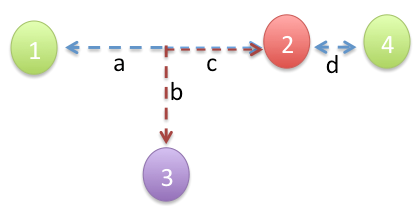
\includegraphics[width=260pt]{../imgs/ej2casos02.jpg}
%\end{center}
\end{minipage}
\hfill
  \fbox{\begin{minipage}[H]{150pt}
    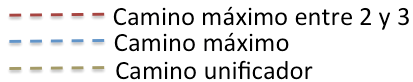
\includegraphics[width=150pt]{../imgs/leyendacasosej2.jpg}
  \end{minipage}}
\caption{Segundo caso posible.}
\end{figure}

A partir del gráfico anterior, supongamos que el camino rojo representa al máximo que resulta del algoritmo $BFS$ luego de haberlo aplicado sobre el nodo 2. \newline
Por otro lado, supongamos que dicho algoritmo retorna al nodo 3 como el más lejano del 2. Como el nodo 3 se encuentra más lejos del 2 que el 1, $b \geq a$. 
\begin{itemize}
\item $a$ = $b$: En este caso, ambos caminos hubieran sido correctos ya que dist(4,1) sería igual a dist(4,3). 
\item $a<b$: Si este caso sucediera, $b$ debería formar parte del camino máximo del árbol. Esto se debe a que el camino más largo del árbol debe estar conformado por los caminos $c$-$d$ y el máximo entre $a$ y $b$. Por lo tanto, si $b>a$, el camino azul no sería el máximo. Luego, es absurdo suponer que el extremo del camino máximo retornado por $BFS$ no pertencía al camino máximo del árbol.\newline
\end{itemize}
\item Tanto el nodo inicial como el final no pertenecen al camino máximo del árbol. \newline \newline
Sea el camino $azul$ el máximo del árbol cuyos extremos son los nodos 1 y 4. Supongamos que el camino $rojo$ representa al camino devuelto por $BFS$ al aplicarlo sobre el nodo 2. En este caso, tenemos dos opciones posibles: El camino $azul$ comparte un tramo con el camino $rojo$ o no comparte ninguno. Veamos cada una de ellas por separado. \newline
\begin{itemize}
\item El camino azul comparte un tramo con el camino rojo. \newline
\begin{figure}[H] %[h] Aqui [b] para button [t] para top
%\begin{center}
\begin{minipage}[H]{240pt}
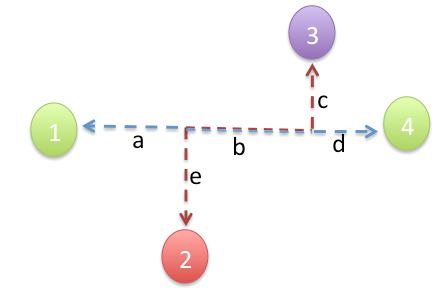
\includegraphics[width=240pt]{../imgs/ej2casos01.jpg}
\end{minipage}
\hfill
  \fbox{\begin{minipage}[H]{150pt}
    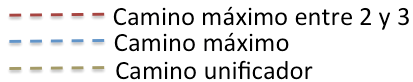
\includegraphics[width=150pt]{../imgs/leyendacasosej2.jpg}
  \end{minipage}}
\caption{Tercer caso posible.}
%\end{center}
\end{figure}
Supongamos que el algoritmo $BFS$ devuelve el nodo 3 como el más alejado al 2. Entonces, podemos deducir que:
\begin {itemize}
\item $c$ = $d$: Ambas soluciones son correctas.
\item $c > d$: Si este caso ocurriera, $c$ debería formar parte del camino máximo del árbol. Luego, el camino azul no sería el máximo. Por lo tanto, resulta absurdo suponer que el extremo del camino máximo otorgado por $BFS$ no pertencía al camino máximo del árbol. \newline
\end{itemize}
\item El camino azul no comparte nigún tramo con el rojo.
\begin{figure}[H] %[h] Aqui [b] para button [t] para top
%\begin{center}
\begin{minipage}[H]{240pt}
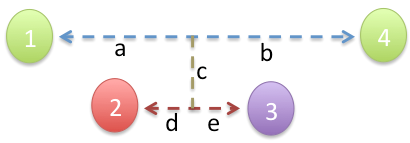
\includegraphics[width=240pt]{../imgs/ej2casos03.jpg}
\end{minipage}
\hfill
  \fbox{\begin{minipage}[H]{150pt}
    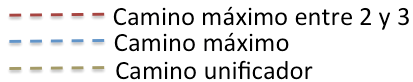
\includegraphics[width=150pt]{../imgs/leyendacasosej2.jpg}
  \end{minipage}}
\caption{Cuarto caso posible.}
%\end{center}
\end{figure}
\end{itemize}
\end{itemize}

Supongamos que el algoritmo $BFS$ nos devuelve el nodo 3 como el más alejado del 2. Entonces, podemos deducir que:
\begin {itemize}
\item $(a \cup c)$ = $e$: Ambas soluciones son correctas.
\item $(b \cup c)$ = $e$: Ambas soluciones son correctas.
\item $(a \cup c) < e$: Si este caso sucediera, $e \cup c$ debería formar parte del camino máximo del árbol. Pero entonces el camino azul no sería el máximo, lo que resulta absurdo.
\item $(b \cup c) < e$: En este caso, $e \cup c$ debería formar parte del camino máximo del árbol. Luego, resulta absurdo.
\newline
\end{itemize}
\end{itemize}

Luego, logramos demostrar que la primera ejecución de $BFS$ retorna como resultado una hoja del árbol al que se le aplica. Además, probamos que dicha hoja pertenece obligatoriamente al camino máximo. Por lo tanto, podemos concluir que la primera ejecución devuelve uno de los dos extremos del camino más largo del árbol. \newline
\newline
\textbf{La segunda ejecución nos devuelve el camino más largo del árbol.} \newline

A la segunda ejecución del algoritmo le ingresa por párametro uno de los extremos del camino más largo del árbol. Luego de dicha ejecución, se obtiene entonces el otro extremo. Una vez encontrado el camino más largo, éste debe ser recorrido hasta hallar el nodo intermedio.
\subsubsection{Complejidad del algoritmo}

Sea $n$ la cantidad de servidores que posee una red de entrega de contenidos (nodos) y $m$ la cantidad de enlaces que los unen (aristas). Dado que procesamos un árbol, sabemos que $m$ = $n-1$, en particular, $m \leq n$.\newline

Para analizar la complejidad de nuestro algoritmo, vamos a calcular la complejidad del algoritmo $BFS$.
\newline

Lo primero que hace $BFS$ es crear dos arreglos de tamaño $n$, uno para almacenar las distancias y el otro para ir marcando los nodos por los cuales ya ocurrió. Crear ambos arreglos tiene una complejidad de $\mathcal{O}(n)$. Además se encola, mediante la función $push$\footnote{http://www.cplusplus.com/reference/queue/queue/push/}, el primer elemento. La complejidad de esta función es $\mathcal{O}(1)$ ya que la estructura interna de la cola está implementada sobre $double-ended\ queue$ y su función $push\_back$ tiene complejidad $\mathcal{O}(1)$.
\newline

Posteriormente, se ingresa a un ciclo que se ejecuta mientras la cola no se encuentre vacía. Esto se controla utilizando la función $empty$\footnote{http://www.cplusplus.com/reference/queue/queue/empty/} cuya complejidad es de $\mathcal{O}(1)$.
\newline

Una vez dentro del ciclo, se aplica la función $front$\footnote{http://www.cplusplus.com/reference/queue/queue/front/} sobre la cola para poder obtener el valor del primer nodo. Luego se usa la función $pop$\footnote{http://www.cplusplus.com/reference/queue/queue/pop/} para quitar este valor de la cola. Ambas funciones tienen una complejidad constante. \newline

Por ultimo, se ejecuta un ciclo el cual recorre un vector de nodos adyacentes. Para cada uno de estos nodos, el algoritmo se fija si fue marcado o no. En caso afirmativo, aplica inserciones sobre arreglos con un $push$; Por lo tanto, dentro del ciclo la complejidad es constante.

Como podemos observar, el ciclo principal se ejecuta $n$ veces ya que todos los nodos son colocados una sola vez en la cola. Además, dentro de este se encuentra otro bucle el cual recorre todos los nodos adyacentes a cada vértice. Es por esto que en el ciclo principal se terminan recorriendo $m$ aristas en las $n$ iteraciones . Por lo tanto la complejidad del ciclo principal es de $\mathcal{O}(n)$ + $\mathcal{O}(m)$ que es igual a $\mathcal{O}(n)$.
\newline

En resumen, el ciclo principal tiene complejidad $\mathcal{O}(n)$ y las funciones que se encuentran antes que este, tienen complejidad $\mathcal{O}(n)$ por lo tanto, la complejidad del algoritmo es $\mathcal{O}(n)$

\subsubsection{Instancias posibles}

Para verificar la correctitud de nuestro programa, dispusimos variar estratégicamente las instancias de entrada al ejecutarlo.
\begin{itemize}
\item En primer lugar, ejecutamos el programa ingresando un caso con una única arista. De este modo, logramos corroborar el correcto funcionamiento de nuestro algoritmo para este tipo de casos borde.\newline
\textbf{Parámetro de entrada:} $$2\ \ 1 $$
$$1\ \ 2\ \ 13 $$
\textbf{Parámetro de salida:} $$13\ \ 2\ \ 1\ \ 1\ \ 2$$

\item Posteriormente, ejecutamos el programa ingresando un solo nodo. De esta forma, pudimos controlar que ocurría si no se ingresaban aristas.\newline
\textbf{Parámetro de entrada:} $$1\ \ 0 $$
\textbf{Parámetro de salida:} $$0\ \ 1\ \ 0$$

\item Por otra parte, quisimos ver un caso que minimizara los costos en el primer ítem pero que ralentizara, luego, el trabajo del $máster$. Este caso nos permite ver que no siempre es mejor elegir el camino mínimo antes que el $máster$, sino que depende lo que se priorice (en este caso el costo final).\newline
\begin{figure}[H] %[h] Aqui [b] para button [t] para top
\begin{center}
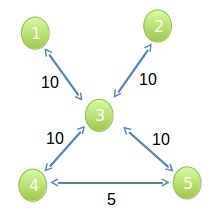
\includegraphics[width=140pt]{../imgs/caso1-ej2.png}
\end{center}
\caption{Grafico de entrada.}
\end{figure}
\textbf{Parámetro de entrada:} $$5\ \ 5$$
$$1\ \ 3\ \ 10$$
$$3\ \ 2\ \ 10$$
$$3\ \  4\ \  10$$
$$3\ \  5\ \  10$$
$$4\ \  5\ \  5$$
\textbf{Parámetro de salida:} $$35\ \ 3\ \ 4\ \ 4\ \ 5\ \ 1\ \ 3\ \ 3\ \ 2\ \ 3\ \ 4 $$

\item También, buscamos una situación inversa al caso anterior, es decir, en el que la elección de conexiones con menor costo permitiera, luego, encontrar un $máster$ eficiente.\newline
\begin{figure}[H] %[h] Aqui [b] para button [t] para top
\begin{center}
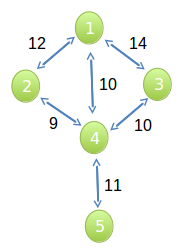
\includegraphics[width=140pt]{../imgs/caso2-ej2.png}
\end{center}
\caption{Grafico de entrada.}
\end{figure}
\textbf{Parámetro de entrada:} $$5\ \  6$$
$$1\ \  2\ \  12$$
$$1\ \  3\ \ 14$$
$$1\ \  4\ \  10$$
$$2\ \  4\ \ 9$$
$$3\ \  4\ \  10$$
$$4\ \  5\ \ 11$$
\textbf{Parámetro de salida:} $$40\ \ 4\ \ 4\ \ 2\ \ 4\ \ 1\ \ 4\ \ 3\ \ 4\ \ 4\ \ 5$$

\item Para finalizar, buscamos un caso que tuviera varias soluciones óptimas en el primer ítem pero que, cada una de estas, implique un costo de replicación de datos distintos (segundo ítem).\newline
\begin{figure}[H] %[h] Aqui [b] para button [t] para top
\begin{center}
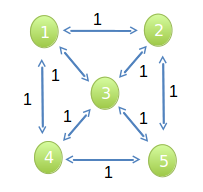
\includegraphics[width=140pt]{../imgs/caso3-ej2.png}
\end{center}
\caption{Grafico de entrada.}
\end{figure}
\textbf{Parámetro de entrada:} $$5\ \ 8$$
$$1\ \ 2\ \ 1$$
$$2\ \ 3\ \ 1$$
$$3\ \ 4\ \ 1$$
$$4\ \ 1\ \ 1$$
$$5\ \ 1\ \ 1$$
$$5\ \ 2\ \ 1$$
$$5\ \ 3\ \ 1$$
$$5\ \ 4\ \ 1$$
\textbf{Parámetro de salida:} $$4\ \ 2\ \ 4\ \ 1\ \ 2\ \ 2\ \ 3\ \ 3\ \ 4\ \ 5\ \ 1$$

\end{itemize}

De este modo, logramos abarcar los casos límite en los que la implementación pudiera haber encontrado algún problema. Dado que los resultados obtenidos fueron los esperados, determinamos que para todas las instancias válidas posibles de entrada nuestra implementación resulta correcta.

\subsubsection{Experimentación}

Para las pruebas de complejidad empírica, generamos instancias aleatorias de costos de los enlaces y servidores variando la cantidad de los mismás. Estas instancias fueron generadas en $C++$ con la función $rand()$ que recibe como parametro una semilla generada por bash. La cantidad de trabajos generados se comprendió entre 200 y 46800, agregando de a 200 en cada iteración. Las mediciones de tiempo en microsegundos se realizaron con la función $high\ resolution\ clock$\footnote{http://en.cppreference.com/w/cpp/chrono/high\_resolution\_clock} de la librería $Chrono$ de $C++$. Debido a que éstas fueron realizadas en microsegundos, las pruebas cuyo tamaño de la entrada era menor a 200 se realizaba en mayor tiempo que las instancias más grandes pues el procesador le otorga más atención al no realizar cambio de contexto. De este modo, logramos medir las pruebas de nuestro algoritmo para comprobar que la complejidad correspondiera con la mencionada anteriormente.

Las funciones de complejidad con las que se compararon nuestros gráficos de tiempo fueron ajustadas por algoritmos matemáticos (proporcionados por \textbf{sci davis}). Dichos algoritmos se encargaron de multiplicarle y sumarle constantes a las funciones con el fin de que éstas se ajustaran a nuestros resultados sin modificar el comportamiento de las funciones utilizadas para comparar.

En este caso, el único valor que puede ser considerado para las ejecuciones es la cantidad de nodos dado que el algoritmo toma, como parámetros de entrada, grafos de tipo árbol. Luego, la cantidad de aristas está definida de acuerdo a la cantidad de nodos del árbol. Es por ello que la variación de otro tipo de parámetro no resultaría relevante para experimentar. Por lo tantoejecutamos el algoritmo con números aleatorios entre $1$ y $150$ correspondientes a los pesos de las aristas.

\begin{figure}[H]
\begin{center}
	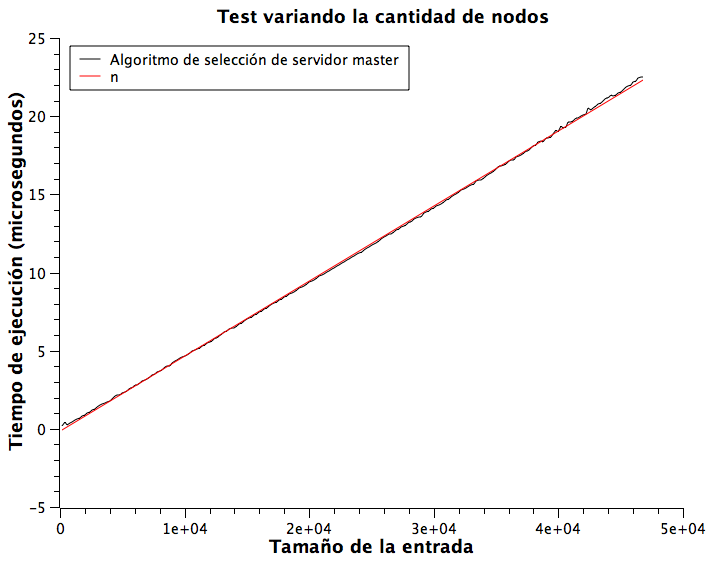
\includegraphics[width=350pt]{../tests/ej2/EJ2-nodo-var.png}
\end{center}
\end{figure}

Podemos apreciar que la complejidad resultante se adapta perfectamente a los valores de entrada.\\

La función utilizada para aproximar nuestros valores resultantes luego de las distintas ejecuciones fue $a*x+b$.
En este caso, los valores que aproximan la función a nuestros datos son:

$$desde\ x = 200\ a\ x = 46.800$$
$$A  = 0,000480693152246956$$
$$B  = -0,176228394042768$$


\subsection{Preguntas adicionales}

\subsubsection{Pregunta 1}
En primer lugar, mostremos un contraejemplo en el que se pueda ver que es posible resolver las dos partes por separado de manera óptima pero que aún así haya una solución en la que la replicación termine en menos tiempo.\newline
\newline
Supongamos que tenemos el siguiente grafo:\newline

\textbf{Formato de entrada:}
$$5\ 5$$
$$4\ \ 3\ \ 1$$
$$5\ \ 3\ \ 1$$
$$3\ \ 2\ \ 1$$
$$1\ \ 5\ \ 1$$
$$3\ \ 1\ \ 1$$

\begin{figure}[H] %[h] Aqui [b] para button [t] para top
\begin{center}
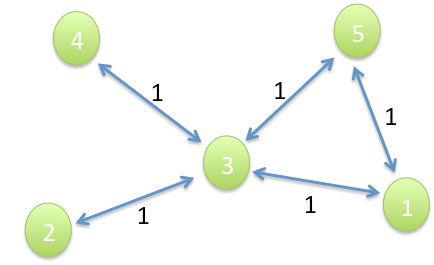
\includegraphics[width=250pt]{../imgs/pregAdicional01.jpg}
\caption{Pregunta 1 - entrada.}
\end{center}
\end{figure}
\newline
Ahora ejecutemos nuestro programa y veamos qué es lo que nos devuelve. \newline


\textbf{Formato de salida:}
$$4\ 5\ 4\ 4\ 3\ 5\ 3\ 3\ 2\ 1\ 5$$

\begin{figure}[H] %[h] Aqui [b] para button [t] para top
\begin{center}
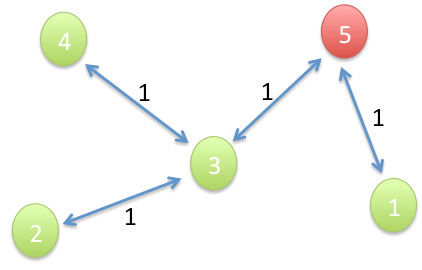
\includegraphics[width=250pt]{../imgs/pregAdicional02.jpg}
\caption{Pregunta 1 - salida.}
\end{center}
\end{figure}

\newline
Como podemos observar en el gráfico anterior, el nodo $máster$ es el 5 y el costo de replicación es igual a 2. Otra solución posible hubiera sido la que tiene al 3 como nodo $máster$ ya que ésta también tiene costo de replicación 2. \newline
\newline
Analicemos por qué nuestro algoritmo devolvió dicha solución. En primer lugar, el árbol generador mínimo ($AGM$) retornado, se encuentra conformado por las primeras cuatro aristas que ingresamos como parámetro de entrada. Ésto se debe a que nuestro algoritmo ordena primero las aristas por su peso y luego toma las menores para generar el $AGM$. En este caso, como todas las aristas tienen el mismo peso, el algoritmo no cambia su orden y genera el $AGM$ con las primeras cuatro. \newline
\newline
Ahora veamos qué ocurre si cambiamos el orden de las aristas:

\textbf{Formato de entrada:}
$$5\ 5$$
$$4\ \ 3\ \ 1$$
$$5\ \ 3\ \ 1$$
$$3\ \ 2\ \ 1$$
$$3\ \ 1\ \ 1$$
$$1\ \ 5\ \ 1$$

\newline
Para ello, cambiemos de lugar las cuarta y quinta aristas: \newline

\textbf{Formato de salida:}
$$4\ 3\ 4\ 4\ 3\ 5\ 3\ 3\ 2\ 3\ 1$$

\begin{figure}[H] %[h] Aqui [b] para button [t] para top
\begin{center}
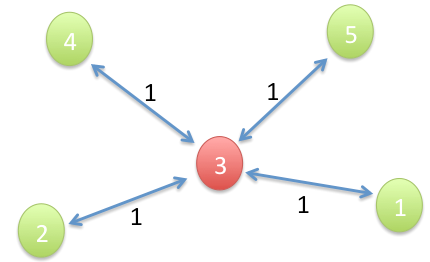
\includegraphics[width=250pt]{../imgs/pregAdicional03.jpg}
\caption{Pregunta 1 - salida2.}
\end{center}
\end{figure}

\newline
Al realizar dicho cambio, el $AGM$ resultante varía. Esto se debe a que, nuevamente, nuestro algoritmo lo genera con las primeras 4 aristas. Sin embargo, esta distribución sigue siendo solución de nuestro problema ya que el costo de sus aristas sigue siendo 4. \newline
Ahora, observemos qué sucede con nuestro nodo $máster$. El nodo máster que nos da esta solución es 3, que también era una posible solución del $AGM$ anterior. La única diferencia con la solución anterior es que, ahora, nuestro costo de replicación es igual a 1, lo que significa que éste es menor. \newline
\newline
Este es un claro ejemplo de un grafo que se resolvió dos veces de manera óptima pero cuya solución inicial indició de distinto modo en la solución del segundo ítem, donde la diferencia culminó en el orden de ingreso de los parámetros.
\newline
\newline
En términos generales, esto puede ocurrir para cualquier grafo en el que la solución del $ítem\ a$ (aplicar el algoritmo de Kruskal) no sea única. Esto se debe a que de todas las soluciones óptimás para el $ítem\ a$ y para cada una de estas, se va a encontrar la solución optima para el $ítem\ b$. Al hacer esto, vamos a encontrar un subconjunto de las soluciones posibles del  $ítem\ a$ que van a tener un menor costo de replicación que las demás.
\newline
\newline
Dos posibles soluciones a esto serian:
\begin{itemize}
\item Para todas las soluciones posibles del  $ítem\ a$, calcular el $ítem\ b$ y me quedo con la que me de menor costo de replicación.
\item Modificar el  $ítem\ a$ para que ordene primero por peso de la arista y luego por la cantidad (de mayor a menor) de nodos adyacentes que tienen ambos extremos de esta. 
\end{itemize}

\subsubsection{Pregunta 2}

 Por otro lado, veamos de qué modo puede modificarse la solución si en lugar de transmitir por $broadcast$ se lo hace por $multicast$, enviando un paquete a cada destino sin hacer copias. \newline

 La principal diferencia entre uno y otro radica en que el primero ($broadcast$) con mandar una vez la informacion le alcanza, ya que cada servidor se guarda y enviá una copia, mientras que el segundo lo que hace es enviar una copia a cada nodo, por lo que realizar un envío de un nodo $a$ a un nodo $b$ cuesta la sumatoria del costo de cada arista del camino. \newline

 Dicho lo anterior, una posible solución priorizando el costo de envió de datos es: \newline

\begin{algorithm}[H]
	\SetAlgoLined
	\caption{Minimización de Caminos entre Fábricas y Clientes}
	\KwIn{Grafo $G$}
	\KwOut{Grafo}
	\ \ \textbf{Grafo} Gmin \\
	\ \ \textbf{Entero} pesoMin = 0 \\
	\ \ \textbf{Mientras}(n \in Nodos(G)) \\
				\ \ \ \ \textbf{Grafo} G' = $Dijktra$(n,G) \\
				\ \ \ \ \textbf{Si} (pesoMin $\leq$ pesoTotal(G')) \\
	      \ \ \ \ \ \ \ Gmin = G' \\
	      \ \ \ \ \ \ \ pesoMin = pesoTotal(G') \\
				\ \ \ \ \textbf{FinSI} \\
		\ \ \textbf{FinMientras} \\
		\ \ \textbf{return} Gmin 
\end{algorithm}

Donde $pesoTotal$ calcula la sumatoria del peso de todas las aristas y  $Dijktra$\footnote{Cormen, Thomas H., Charles E. Leiserson, and Ronald L. Rivest. p.658} calcula los caminos mínimos de un nodo hasta todos los demás. De esta manera nos vamos quedando con aquella solución que la sumatoria de todas las aristas posea menor peso. \newline

Esta solución tiene una complejidad de $\mathcal{O}(n^{3})$ siendo n la cantidad de servidores (nodos), ya que por cada vértice aplica dicho algoritmo.\newline

\newpage

\section{Ejercicio 3}
\subsection{Problema a resolver}
El siguiente problema consiste en realizar un algoritmo capaz de resolver problemas de caminos mínimos con ciertas particularidades. El mismo radica en una empresa productora de ladrillos cuyas fábricas se encuentran en distintos lugares de una provincia, al igual que sus clientes. Para transportar los ladrillos entre las fábricas y los clientes, la empresa debe encargarse de fortalecer las rutas por las que se trasladan sus camiones. Dichas rutas tienen un costo de inversión proporcional a la longitud de las mismas. Luego, la empresa desea replanificar sus recorridos a modo de minimizar los gastos que implican los fortalecimientos de las rutas a utilizar. Para ello, la empresa debe asegurarse de que exista un camino fortalecido entre cada cliente y al menos una de sus fábricas. Debe considerarse que desde todas las fábricas sale al menos una ruta, que los costos de inversión son enteros positivos, que es posible satisfacer la demanda de cada cliente y que no hay más fábricas que clientes.

Los formatos de entrada y salida del problema son los que siguen:\newline


\textbf {Formatos de entrada y salida:}\newline
\newline
La entrada contiene varias instancias del problema. La primera línea de cada instancia contiene los siguientes valores (enteros positivos, separados por un espacio):

$$F\ C\ R$$

donde \textbf{$F$} indica la cantidad de fábricas de la empresa (numeradas de 1 a \textbf{$F$}), \textbf{$C$} indica la cantidad de clientes (numerados de \textbf{$F+1$} a \textbf{$F+C$}) y \textbf{$R$} indica la cantidad de rutas de la provincia. A esta línea le siguen \textbf{$R$} líneas y cada una de ellas describe una de las rutas de la provincia. Para cada ruta, la línea correspondiente contiene los siguientes valores (enteros positivos, separados por un espacio):

$$e_{1}\ e_{2}\ l$$

donde \textbf{$e_{1}$} y \textbf{$e_{2}$} son los extremos de la ruta y \textbf{$l$} es la longitud de la misma. Los extremos de la ruta pueden ser fábricas y/o clientes y son números enteros en el rango [1,\textbf{$F+C$}]. La entrada concluye con una línea comenzada por 0.\newline

La salida debe contener una línea por cada instancia de entrada. Esta línea debe contener los siguientes valores (separados por un espacio):

$$L\ k\ e_{1}^1\ e_{2}^1\ e_{1}^2\ e_{2}^2\...\ e_{1}^k\ e_{2}^k$$

donde \textbf{$L$} es el costo total de la solución (la suma de las longitudes de las rutas utilizadas), $k$ es la cantidad de rutas utilizadas en la solución y $e_{1}^i$ y $e_{2}^i$ son los extremos de la $i$-ésima ruta utilizada, para $i\ \in$ [1,$k$].\newline

En lo que sigue, presentaremos dos ejemplos del problema a resolver:
\begin{itemize}
\item {\large{\textbf{Ejemplo 1:}}}\newline
\newline
En el ejemplo que sigue, decidimos mostrar un clásico caso del problema. En éste, se puede observar que, si bien existe más de una ruta entre cada cliente y alguna fábrica, la solución devuelve una sola ruta para cada uno de ellos.\newline
\newline
\textbf{Formato de entrada:}

$$3\ \ 5\ \ 8$$
$$1\ \ 4\ \ 40$$
$$1\ \ 5\ \ 40$$
$$4\ \ 5\ \ 100$$
$$1\ \ 6\ \ 70$$
$$6\ \ 7\ \ 100$$
$$7\ \ 2\ \ 70$$
$$2\ \ 8\ \ 40$$
$$3\ \ 8\ \ 40$$

\begin{figure}[H] %[h] Aqui [b] para button [t] para top
\begin{center}
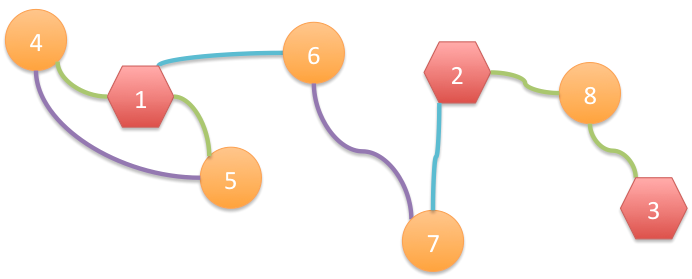
\includegraphics[width=350pt]{../imgs/ejemplo1ej3ent.jpg}
\end{center}
\fbox{\begin{minipage}[H]{90pt}
    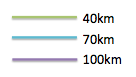
\includegraphics[width=90pt]{../imgs/leyendaej3.jpg}
  \end{minipage}}
  \hfill
  \fbox{\begin{minipage}[H]{60pt}
    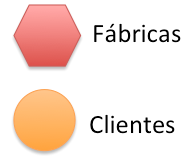
\includegraphics[width=60pt]{../imgs/leyendaformas.jpg}
  \end{minipage}}
\caption{Ejemplo 1 - entrada.}
\end{figure}

\textbf{Formato de salida:}
$$260\ \ 5\ \ 1\ \ 4\ \ 1\ \ 5\ \ 2\ \ 8\ \ 1\ \ 6\ \ 7\ \ 2$$

\begin{figure}[H] %[h] Aqui [b] para button [t] para top
\begin{center}
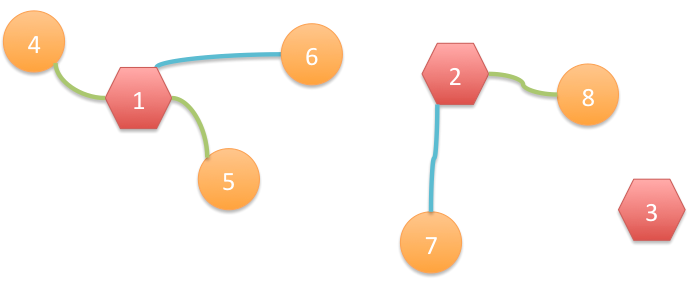
\includegraphics[width=350pt]{../imgs/ejemplo1ej3sal.jpg}
\caption{Ejemplo 1 - salida.}
\end{center}
\end{figure}
\item {\large{\textbf{Ejemplo 2:}}}\newline
\newline
En este ejemplo, puede verse que si bien todos los clientes se encuentran conectados a una fábrica de forma directa, las rutas elegidas son las indirectas dado que la suma de éstas es inferior a la otra opción. Por otra parte, puede observarse que algunas fábricas resultan inutilizables luego de la minimización de rutas, como ocurre para la fábrica nº1.\newline
\newline
\textbf{Formato de entrada:}

$$2\ \ 4\ \ 7$$
$$3\ \ 4\ \ 20$$
$$5\ \ 6\ \ 20$$
$$4\ \ 5\ \ 20$$
$$2\ \ 3\ \ 90$$
$$2\ \ 4\ \ 70$$
$$2\ \ 5\ \ 50$$
$$2\ \ 6\ \ 20$$
$$1\ \ 6\ \ 70$$

\begin{figure}[H] %[h] Aqui [b] para button [t] para top
\begin{center}
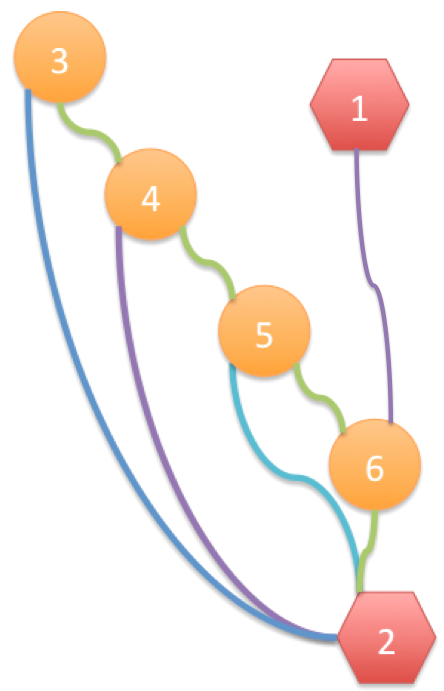
\includegraphics[width=140pt]{../imgs/ejemplo2ej3ent.jpg}
\end{center}
\fbox{\begin{minipage}[H]{70pt}
    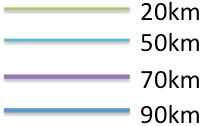
\includegraphics[width=70pt]{../imgs/leyendaej3ejmp2.jpg}
  \end{minipage}}
  \hfill
  \fbox{\begin{minipage}[H]{60pt}
    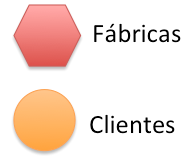
\includegraphics[width=60pt]{../imgs/leyendaformas.jpg}
  \end{minipage}}
\caption{Ejemplo 2 - entrada.}
\end{figure}

\textbf{Formato de salida:}
$$80\ \ 4\ \ 3\ \ 4\ \ 5\ \ 6\ \ 4\ \ 5\ \ 2\ \ 6$$

\begin{figure}[H] %[h] Aqui [b] para button [t] para top
\begin{center}
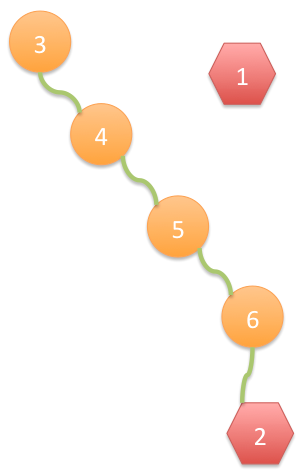
\includegraphics[width=140pt]{../imgs/ejemplo2ej3sal.jpg}
\caption{Ejemplo 2 - salida.}
\end{center}
\end{figure}
\end{itemize}


\subsection{Resolución coloquial}

Antes de explicar la resolución elegida para el problema descrito, formalicemos el modelo a utilizar:
\begin{itemize}
\item  \textbf{Nodos:} Clientes y Fábricas
\item  \textbf{Aristas:} Rutas
\item  \textbf{Pesos de las aristas:} Longitud
\end{itemize}

Luego, cuando hablemos de \textbf{Grafo}, nos vamos a estar refiriendo a una provincia que contiene clientes, fábricas y rutas.\newline

Para resolver este problema, optamos por la utilización de un algoritmo encargado de hallar un Árbol Generador Mínimo. Esto se debe a que buscamos minimizar el costo de reparación de las rutas siempre que se respete la restricción de que todos los clientes se mantengan conectados con al menos una fábrica. Luego, buscamos minimizar el peso de las aristas del grafo.\newline

Al idealizar la resolución del problema, nos encontramos con que puede no existir un camino entre todo par de vértices (un grafo no conexo). Esto nos impidió utilizar los algoritmos vistos en clase dado que aplican sobre grafos conexos. Para solucionar dicho inconveniente, optamos por crear un nodo llamado $ghost$ que se conectara con aristas de peso cero a todas las fábricas. De esta manera, nos aseguramos obtener un grafo conexo ya que todos los clientes se encuentran enlazados con al menos una fábrica y unimos todas las componentes conexas.\newline

Una vez insertado el nodo $ghost$, se ejecuta el algoritmo de $Kruskal$ a fin de hallar un árbol generador mínimo. Luego, la suma de las longitudes de todas las rutas es la menor. Posteriormente, procedemos a eliminar el nodo $ghost$, obteniendo, así, un conjunto de componentes conexas con al menos una fábrica cada una y cuyas sumas de las longitudes de rutas a reparar es la menor posible.\newline

El pseudocódigo que resuelve el problema es el siguiente:\newline

\begin{algorithm}[H]
	\SetAlgoLined
	\caption{Minimización de Caminos entre Fábricas y Clientes}
	\KwIn{Grafo $G$, Precios $ps$}
	\KwOut{Grafo}
	NodoFabrica $ghost$\\
	Agregar(Nodos($G$),$ghost$)\\
	\ForAll{$v \in$ Nodos($G$)}{
		\If{esFabrica($v$) $\land\ v\ \neq\ ghost$}{ \\
			Agregar(aristas($G$),$<v$,$ghost>$)\\
			$ps$[$v$,$ghost$] = $0$ \\
		}
	}
	Kruskal($G$,$ps$) \\
	Filtrar($G$,$ghost$) \\
	\textbf{devolver} $G$	
\end{algorithm}

\begin{algorithm}[H]
	\SetAlgoLined
	\caption{Filtrar}
	\KwIn{Grafo $G$, Nodo $ghost$}
	\ForAll{$v \in$ Nodos($G$)}{
		\If{$v$ \textbf{incide con} $ghost$}{ \\
			\textbf{Eliminar arista} $<v$,$ghost>$\\
		}
	}	
\end{algorithm}

donde $Agregar(Nodos(G),x)$ agrega el nodo $x$ a los nodos de $G$. Por otro lado, $esFabrica(v)$ es una función que devuelve $true$ si $v$ es una fábrica, caso contrario devuelve $false$.

\subsection{Demostración de correctitud}

Demostremos que el algoritmo planteado es correcto. Para ello, veamos que \textbf{se fortalecen las rutas necesarias al menor costo posible}. Donde \textbf{rutas necesarias} hace referencia a un conjunto de rutas tal que existe al menos un camino fortalecido entre un cliente y una fábrica. Por otro lado, \textbf{menor costo posible} hace alusión a que la sumatoria de todos los costos sea el menor posible.\newline

Por un lado, sabemos que \textbf{es posible satisfacer la demanda de todos los clientes} implica que para todo cliente existe un camino que lo une a una fábrica $[1]$.  \newline
\begin{figure}[H] %[h] Aqui [b] para button [t] para top
\begin{center}
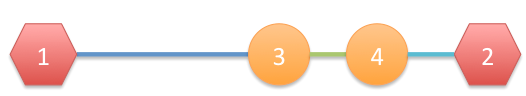
\includegraphics[width=230pt]{../imgs/demo3-1.jpg}
\end{center}
%\fbox{\begin{minipage}[H]{70pt}
%  \end{minipage}}
  \hfill
  \fbox{\begin{minipage}[H]{90pt}
    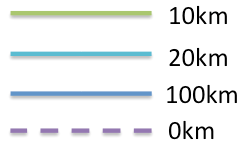
\includegraphics[width=90pt]{../imgs/leyendademo3.jpg}
  \end{minipage}}
  \caption{Ejemplo que muestra que todo cliente se une con al menos una fábrica.}
\end{figure}
\end{itemize}

Luego, queremos probar lo siguiente:
\begin{itemize}
\item Si agregamos aristas adyacentes entre cada fábrica y un nodo $ghost$ $[2]$ y aplicamos el algoritmo de $Kruskal$, el resultado cumple que todos los clientes están conectados con todas las fábricas (pues consiste en un árbol generador) $[3]$. Por otra parte, la sumatoria de todos los costos es igual a la de la solución optima (pues las aristas agregadas tenían peso cero y $Kruskal$ selecciona la sumatoria de costos mínima).

Por lo tanto, obtenemos una solución cuyo peso es mínimo, pero que mantiene las aristas de peso cero.

\begin{figure}[H] %[h] Aqui [b] para button [t] para top
\begin{center}
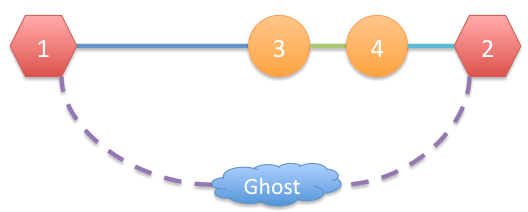
\includegraphics[width=230pt]{../imgs/demo3-2.jpg}
\caption{Ejemplo con el nodo Ghost agregado.}
\end{center}
\end{figure}
\end{itemize}


\item Luego, eliminamos las aristas que inciden en el nodo $ghost$. Dado que éstas tenían peso cero, el costo total de la solución no se ve afectado.

\begin{figure}[H] %[h] Aqui [b] para button [t] para top
\begin{center}
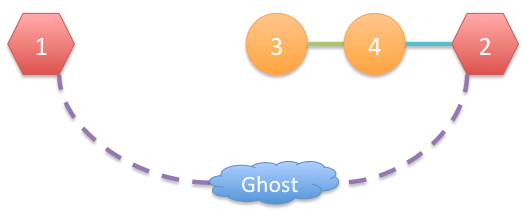
\includegraphics[width=230pt]{../imgs/demo3-3.jpg}
\caption{Ejemplo luego de aplicar el algoritmo de Kruskal.}
\end{center}
\end{figure}
\end{itemize}

\item Por último, debemos asegurarnos de que todas las componentes conexas restantes poseen al menos una fábrica. Esto se cumple ya que, por $[1]$ todas las componentes tienen al menos una fábrica, por $[3]$ todas las fábricas y clientes están conectados y, por $[2]$, las aristas eliminadas inciden sólo en fábricas, por lo que eliminarlas no descarta caminos entre clientes y éstas.

\begin{figure}[H] %[h] Aqui [b] para button [t] para top
\begin{center}

\includegraphics[width=230pt]{../imgs/demo3-4.jpg}
\caption{Ejemplo luego de eliminar las aristas de costo cero.}
\end{center}
\end{figure}
\end{itemize}

De este modo, a partir de las rutas, fábricas y clientes ingresados como parámetro de entrada, logramos obtener el conjunto de rutas cuya suma de costos es mínima logrando que cada cliente se encuentre conectado a una fábrica, siendo ésto lo que buscábamos.

\end{itemize}

\subsection{Complejidad del algoritmo}

 En esta sección, detallaremos la complejidad de nuestro algoritmo junto con la justificación de la elección de cada estructura. 

En principio, para definir el grafo ingresado por parámetro, utilizamos un $vector<Arista>$, donde $Arista$ es un struct que posee tres enteros (su peso y los nodos que conecta), y dos enteros que representan la cantidad de clientes y de fábricas. Para definir dicha estructura, reservamos ($reserve$\footnote{http://es.cppreference.com/w/cpp/container/vector/reserve}) el espacio a utilizar por el vector, siendo éste de $R + F$. Esto se debe a que, posteriormente, dicho vector almacena una suma de aristas correspondiente a la cantidad de fábricas y, de este modo, nos aseguramos de que el agregado ($push\_back$\footnote{http://es.cppreference.com/w/cpp/container/vector/push$\_$back}) de las mismas sea $\mathcal{O}(1)$. Luego, el costo de reservar dicha memoria es $\mathcal{O}(R + F)\ \leq\ \mathcal{O}(2R)$ = $\mathcal{O}(R)$, pues $F \leq R$ (por enunciado\footnote{Enunciado: "Se sabe que desde todas las fabricas sale al menos una ruta, que es posible satisfacer la demanda de cada cliente, y que no hay mas fabricas que clientes"}). De este modo, el cargado de la entrada se realiza en forma lineal respecto de la cantidad de elementos, es decir, las aristas ($R$).

 Una vez realizado esto, se comienza con la resolución del problema. Cabe aclarar que todas las funciones toman los valores por referencia, de esta manera se evitan copias innecesarias. Lo primero que realizamos es la incorporación de un nodo. Esto es constante pues consiste en sumarle uno a $cant\_nodos$ y retornar el valor obtenido. Luego, se incorporan las aristas incidentes al nodo $ghost$. Dicho proceso se realiza en tiempo lineal con respecto a la cantidad de fábricas ya que las recorre, crea una arista y la inserta en el vector (crear una arista es constante al igual que insertar el nodo pues el espacio se encontraba reservado previamente). Luego, la cantidad de rutas pasa a ser $R+F$.

 Posteriormente, se prosigue aplicando el algoritmo de $Kruskal$ cuyo costo temporal es $\mathcal{O}(m^*log(n))$\footnote{Dicha complejidad se encuentra detallada en la sección $2.1$ dado que se utilizó exactamente el mismo algoritmo.} donde $m$ = $R+F$ y $n$ = $F+C$.

 Luego del algoritmo de $Kruskal$, se realiza el llamado a la función $filtrar$. Ésta comienza con la función $reserve$ ($\mathcal{O}(n)$)\footnote{http://www.cplusplus.com/reference/vector/vector/reserve/} que reserva la cantidad de rutas menos la cantidad de fábricas, luego $R+F$-$F$ = $R$ lugares en el vector. A continuación, se recorren todas las aristas $R+F$ almacenando, en cada paso, las arista no incidentes en el nodo $ghost$ en el vector creado anteriormente. Dicha comparación es constante ya que sólo se accede a un par de aristas. Por último, se le resta uno a la cantidad de nodos ($\mathcal{O}(1)$) permitiéndonos concluir que la complejidad final de esta función resulta $\mathcal{O}(R+F)$ = $\mathcal{O}(R)$.

 Finalmente, podemos concluir que la complejidad resulta $\mathcal{O}(R)$ + $\mathcal{O}(F)$ + $\mathcal{O}((R+F)log(F+C))$ + $\mathcal{O}(R)$ + $\mathcal{O}(R)$ =  $\mathcal{O}((R+F)log(F+C))$ = $\mathcal{O}(2^*R^*log(2C))$ = $\mathcal{O}(2^*log(2)^*R^*log(C))$ = $\mathcal{O}(R^*log(C))$ dado que $F \leq C \leq R$.


\subsection{Instancias posibles}
Para verificar la correctitud de nuestro programa, dispusimos variar estratégicamente las instancias de entrada al ejecutarlo.
\begin{itemize}

\item En primer lugar, ingresamos una instancia que consideramos base. Ésta consiste en una única fábrica conectada a un cliente. Dado que no es posible ingresar el carácter 0 por ser el indicador del final del archivo, no pueden existir casos con valores menores a éste.
De este modo, logramos evaluar un tipo de caso borde.\newline
\textbf{Parámetro de entrada:} $$1\ \ 1\ \ 1$$
$$1\ \ 2\ \ 10$$
\textbf{Parámetro de salida:} $$10\ \ 1\ \ 1\ \ 2$$


\item Por otra parte, probamos ingresando dos clientes y una fábrica interconectados entre sí. El objetivo de esta instancia es ver que nuestro algoritmo elige, efectivamente, el camino más corto sin importar de qué modo une a los clientes con la fábrica ya que ésto resulta indistinto siempre que la componente conexa la contenga. \newline
\begin{figure}[H] %[h] Aqui [b] para button [t] para top
\begin{center}
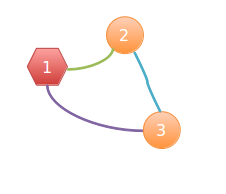
\includegraphics[width=140pt]{../imgs/caso1-ej3.png}
\end{center}
  \hfill
  \fbox{\begin{minipage}[H]{90pt}
    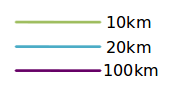
\includegraphics[width=90pt]{../imgs/leyendaformasinstancias.png}
  \end{minipage}}
\caption{Ejemplo de caso con 3 nodos}
\end{figure}
\textbf{Parámetro de entrada:} $$1\ \  2\ \  3$$
$$1\ \  2\ \  10$$
$$1\ \  3\ \  100$$
$$2\ \  3\ \  20$$																											
\textbf{Parámetro de salida:} $$30\ \ 2\ \ 1\ \ 2\ \ 2\ \ 3$$


\item También, quisimos visualizar qué ocurría cuando la entrada tenía varias soluciones posibles. De este modo, logramos ver cuál de las soluciones óptimas elegía nuestro algoritmo.\newline
\begin{figure}[H] %[h] Aqui [b] para button [t] para top
\begin{center}
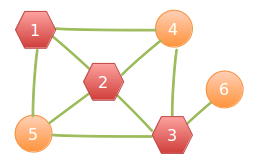
\includegraphics[width=140pt]{../imgs/caso2-ej3.png}
\end{center}
\caption{Ejemplo de varias soluciones}
\end{figure}
\textbf{Parámetro de entrada:} $$3\ \  3\ \  7$$
$$1\ \  4\ \  10$$
$$1\ \  5\ \  10$$
$$2\ \ 5\ \  10$$
$$2\ \ 4\ \  10$$
$$3\ \  5\ \  10$$
$$3\ \  4\ \  10$$
$$3\ \  6\ \  10$$
\textbf{Parámetro de salida:} $$30\ \ 3\ \ 1\ \ 4\ \ 1\ \ 5\ \ 3\ \ 6$$

\item Para finalizar, probamos un caso compuesto por varias componentes no conexas. Para ello, creamos una instancia que posee tres pares de (clientes, fábricas) no conectadas entre ellos. \newline
\begin{figure}[H] %[h] Aqui [b] para button [t] para top
\begin{center}
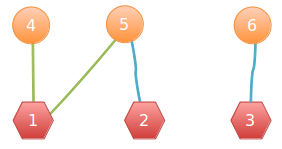
\includegraphics[width=140pt]{../imgs/caso4-ej3.png}
\end{center}
\caption{Ejemplo varias componentes conexas.}
\end{figure}
\textbf{Parámetro de entrada:} $$3\ \  3\ \  4$$
$$1\ \  4\ \  10$$
$$1\ \  6\ \  10$$
$$5\ \  2\ \  20$$
$$3\ \  6\ \  100$$																									
\textbf{Parámetro de salida:} $$40\ \ 3\ \ 1\ \ 4\ \ 1\ \ 6\ \ 5\ \ 2$$

\end{itemize}


De este modo, logramos abarcar los casos límite en los que la implementación pudiera haber encontrado algún problema. Dado que los resultados obtenidos fueron los esperados, determinamos que para todas las instancias válidas posibles de entrada nuestra implementación resulta correcta.


\subsection{Experimentación}
Para las pruebas de complejidad empírica, generamos instancias aleatorias de grafos alterando la cantidad de nodos y aristas. Estas instancias fueron generadas en $C++$ con la función $rand()$. La cantidad de grafos generados se comprendió entre 200 y 100000, agregando de a 200 en cada iteración. Las mediciones de tiempo en nanosegundos se realizaron con la función $high\ resolution\ clock$\footnote{http://en.cppreference.com/w/cpp/chrono/high\_resolution\_clock} de la librería $Chrono$ de $C++$. Debido a que éstas fueron realizadas en nanosegundos, las pruebas cuyo tamaño de la entrada era menor a 200 se realizaba en mayor tiempo que las instancias más grandes pues el procesador le otorga más atención al no realizar cambio de contexto. De este modo, logramos medir las pruebas de nuestro algoritmo para comprobar que la complejidad correspondiera con la mencionada anteriormente.

Las funciones de complejidad con las que se compararon nuestros gráficos de tiempo fueron ajustadas por algoritmos matemáticos (proporcionados por \textbf{sci davis}). Dichos algoritmos se encargaron de multiplicarle y sumarle constantes a las funciones con el fin de que éstas se ajustaran a nuestros resultados sin modificar el comportamiento de las funciones utilizadas para comparar.

El algoritmo que genera las instancias garantiza que siempre va a haber al menos una fabrica conectada directa o indirectamente a un cliente, de forma tal que la instancia no se vuelva invalida.
\newpage
En una primera instancia, generamos grafos aleatorios variando la cantidad de nodos y dejando la cantidad de aristas en un valor fijo. Este valor es un porcentaje de la cantidad máxima de aristas que puede tener el grafo. El porcentaje que elegimos para determinar un grafo denso fue el $50\%$ de la cantidad máxima de aristas que puede tener el grafo. La cantidad de nodos que representan fabricas es del $50\%$.

\begin{figure}[H]
	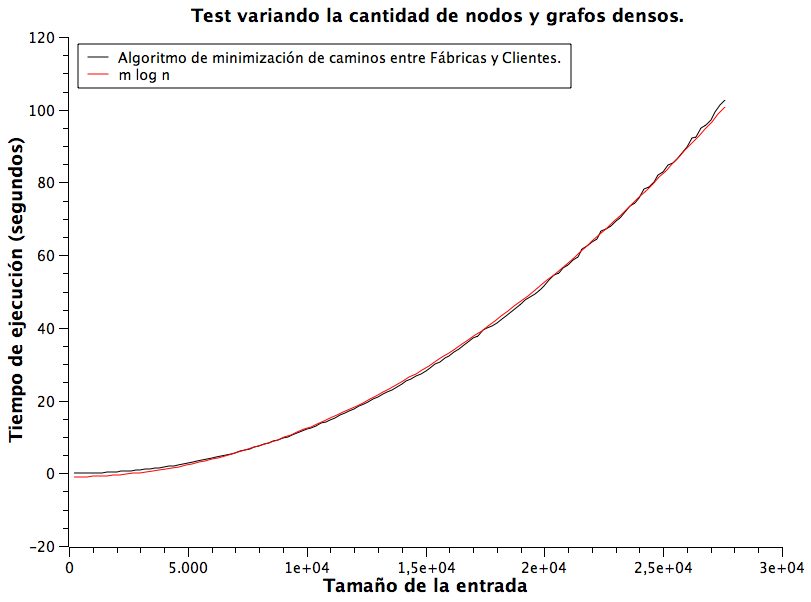
\includegraphics[width=350pt]{../tests/ej3/EJ3-nodo-var-denso.png}
%\end{center}
\end{figure}

En este caso se puede apreciar como la complejidad se adapta perfectamente a los valores de entrada.\\
La función utilizada para aproximar nuestros valores resultantes luego de las distintas ejecuciones fue $$a*(((20*(x*(x-1)/2)) / 100) + log(x)) + b$$.
En este caso, los valores que aproximan la función a nuestros datos son:

$$desde\ x = 200\ a\ x = 27.600 $$
$$a  = 1,33661247156849e-06$$
$$b  = -1,01492247788281 $$

\newpage
Luego generamos un lote de pruebas pero para grafos livianos, estos a diferencia de los anteriores tienen $5\%$ de aristas y $5\%$ de nodos que representan fabricas.

\begin{figure}[H]
	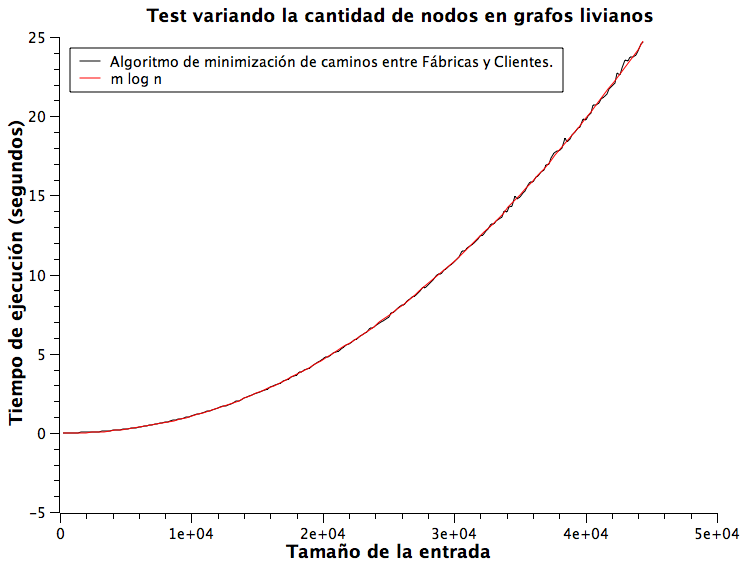
\includegraphics[width=350pt]{../tests/ej3/EJ3-nodo-var-liviano.png}
%\end{center}
\end{figure}

En este caso se puede apreciar como la complejidad se adapta perfectamente a los valores de entrada. Respecto al caso anterior, los tiempos de ejecución son mas rápidos con lo cual se pudieron realizar mayor cantidad de pruebas. Esto deja en evidencia que la cantidad de aristas impacta directamente en la complejidad, tal como mostramos en el análisis del mismo.\\
La función utilizada para aproximar nuestros valores resultantes luego de las distintas ejecuciones fue $$ a*(((20*(x*(x-1)/2)) / 100) + log(x)) + b $$.
En este caso, los valores que aproximan la función a nuestros datos son:

$$desde\ x = 200\ a\ x = 44.400 $$
$$a  = 2,70030174291421e-08$$
$$b  = -0,0228951001523759 $$


\newpage
Luego, generamos un lote de grafos cuya cantidad de nodos esta fija, y variamos la cantidad de aristas entre 1 y 100 por ciento sobre la capacidad máxima de aristas que puede soportar el grafo. La cantidad de nodos que elegimos para este grafo es de $3000$. La cantidad de fabricas en este caso definido como denso es del $20\%$.

\begin{figure}[H]
	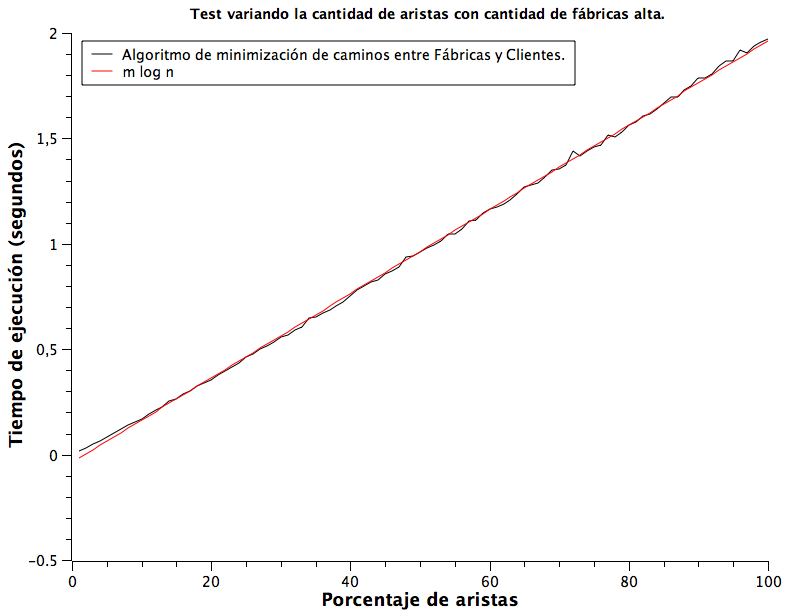
\includegraphics[width=350pt]{../tests/ej3/EJ3-r-var-denso.png}
%\end{center}
\end{figure}

En este caso se puede apreciar como la complejidad se adapta perfectamente a los valores de entrada. Debido a que la función de complejidad fija la parte logarítmica, los valores resultantes se parecen a una función lineal, lo cual tiene sentido ya que la única variable que se modifica a lo largo de las pruebas es lineal.\\
La función utilizada para aproximar nuestros valores resultantes luego de las distintas ejecuciones fue $$a*((x*(3000*(3000-1)/2))/100)*log(3000)+b $$.
En este caso, los valores que aproximan la función a nuestros datos son:

$$desde\ x = 1\ a\ x = 100 $$
$$a  = 1,27748699850107e-07$$
$$b  = -0,0359196477978645 $$

\newpage
Luego, generamos un lote igual al anterior excepto por el porcentaje de fabricas, esto lo hicimos para ver si la complejidad se veía afectada por la cantidad de conexiones de nodos fantasmas que el programa hacia. El porcentaje de fabricas para este caso es de $1\%$.

\begin{figure}[H]
	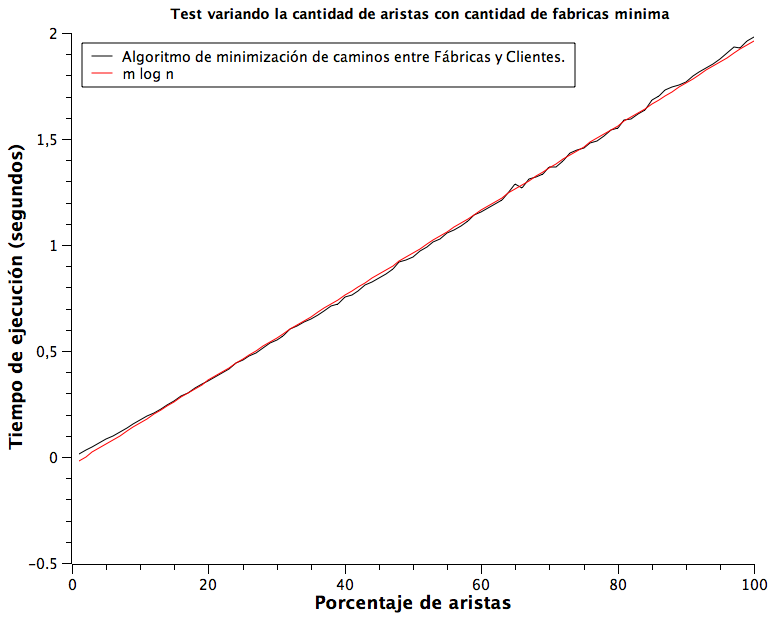
\includegraphics[width=350pt]{../tests/ej3/EJ3-r-var-liviano.png}
%\end{center}
\end{figure}

En este caso se puede apreciar como la complejidad se adapta perfectamente a los valores de entrada, y concluimos que la cantidad de fabricas no modifica la complejidad del algoritmo, siento los tiempos del grafico iguales al anterior.\\
La función utilizada para aproximar nuestros valores resultantes luego de las distintas ejecuciones fue $$ a*((x*(3000*(3000-1)/2))/100)*log(3000)+b$$.
En este caso, los valores que aproximan la función a nuestros datos son:

$$desde\ x = 1\ a\ x = 100$$
$$a  = 1,28059038055647e-07$$
$$b  = -0,038836147808835$$

\newpage 
Finalmente, veamos un caso en el cual quisimos analizar el caso en el cual variáramos la cantidad de nodos que representan fabricas, para ver si esto influía en los tiempos de ejecución del algoritmo. Hicimos dos lotes, en el primero, que definimos como denso, la cantidad de aristas esta en función de la cantidad de nodos, esta cantidad es del $20\%$ y en el segundo lote que definimos como liviano pusimos la mínima cantidad de aristas, siendo esta el mínimo para garantizar que las instancias de los problemas sean validas. La cantidad de nodos de este grafo es de $3000$.

\begin{figure}[H]
	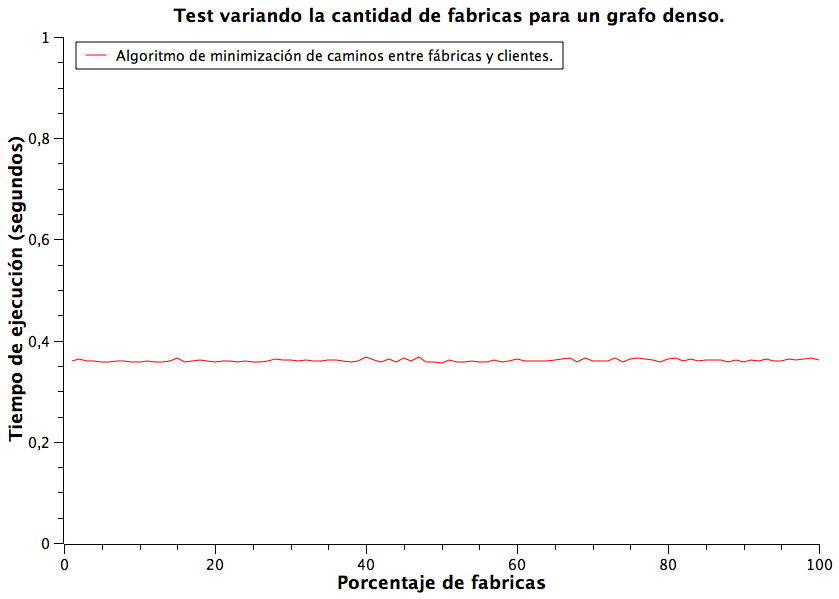
\includegraphics[width=370pt]{../tests/ej3/EJ3-f-var-denso.png}
%\end{center}
\end{figure}

\begin{figure}[H]
	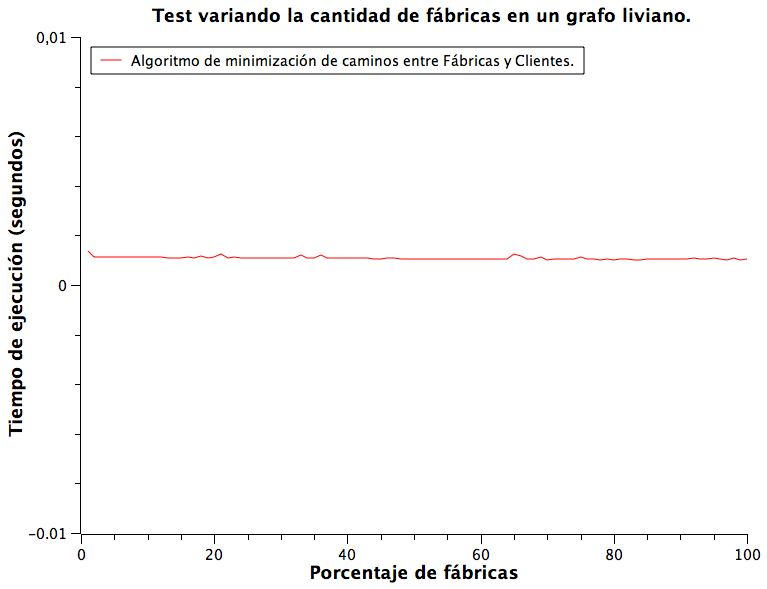
\includegraphics[width=370pt]{../tests/ej3/EJ3-f-var-liviano.png}
%\end{center}
\end{figure}

\newpage


\section{Referencias}
\begin{itemize}
\item CORMEN, THOMAS H. ; Introduction to Algorithms, Third ed. 2009. The MIT Press.
\item http://jariasf.wordpress.com/2012/04/19/arbol-de-expansion-minima-algoritmo-de-kruskal/
\end{itemize}


\section{Código fuente}

\subsection{Ejercicio 1:}

\begin{figure}[H]
\begin{center}
\begin{verbatim}
int sigTrabajo = max(m1, m2)+1; //calculo el siguiente trabajo
if (sigTrabajo > cantTrabajos)
    return 0;
if (matriz[m1][m2]>-1)
    return matriz[m1][m2];
else {
    int costo1 = cs[sigTrabajo-1][m1] + minimizacionDeCostos(sigTrabajo, m2);
    int costo2 = cs[sigTrabajo-1][m2] + minimizacionDeCostos(m1, sigTrabajo);
    if (costo1 < costo2) {
        matriz[m1][m2] = costo1;
        matriz[m2][m1] = costo1;
        return costo1;
    } else {
        matriz[m1][m2] = costo2;
        matriz[m2][m1] = costo2;
        return costo2;
    }
}
\end{verbatim}
\caption{Función de minimización de costos.}

\begin{verbatim}
cout << minimizacionDeCostos(0,0) << " ";

int m1=0, m2=0;
vector<int> maquina1;

for (int i = 1; i < cantTrabajos; ++i)
    if (matriz[i][m2] < matriz[m1][i])
        m1 = i;
    else {
        m2 = i;
        maquina1.push_back(i);
    }

if (cs[cantTrabajos-1][m2] < cs[cantTrabajos-1][m1]) 
    maquina1.push_back(cantTrabajos);
\end{verbatim}
\caption{Inicialización de minimización de costos.}
\end{center}
\end{figure}

\subsection{Ejercicio 2:}

\begin{figure}[H]
\begin{center}
\begin{verbatim}
while (!cola.empty()){
	cabeza = cola.front();
	cola.pop();			
	for (int i = 0; i < listaDeAdyacencia[cabeza-1].size(); i++){
		int nodo = listaDeAdyacencia[cabeza-1][i];	
		if(!loAgregue[nodo-1]){ 
			padre[nodo-1]=cabeza;
			loAgregue[nodo-1] = true;
			distancias[nodo-1] = distancias[cabeza-1] + 1;
			cola.push(nodo);
		}		
	}	
}
	
res.first = cabeza;
	
int nodo = padre[cabeza-1];
int medio = (distancias[cabeza-1])/2;
for (int i = 0; i < cantNodos; i++){
	medio--;
	if (medio <= 0)
		break;
	nodo = padre[nodo-1];
}
	
res.second = nodo;
\end{verbatim}
\caption{BFS.}

\begin{verbatim}
int master (int cantNodos, vector<vector<int> >& listaDeAdyacencia){
	pair<int, int> resDeBFS;
	resDeBFS = bfs(1, cantNodos, listaDeAdyacencia);
	resDeBFS = bfs(resDeBFS.first, cantNodos, listaDeAdyacencia);
	return resDeBFS.second;
}
\end{verbatim}
\caption{Función encargada de buscar el master.}

\begin{verbatim}
res = kruskal(cantNodos, aristas);	
	for (int i = 0; i < res.size(); i++){
		int nodoA = res[i].nodo_a;
		int nodoB = res[i].nodo_b;
		listaDeAdyacencia[nodoA-1].push_back(nodoB);
		listaDeAdyacencia[nodoB-1].push_back(nodoA);
	}
\end{verbatim}
\caption{Función encargada de encontrar el AGM.}
\end{center}
\end{figure}
\subsection{Ejercicio 3:}

\begin{figure}[H]
\begin{center}
\begin{verbatim}
vector<Arista> ej3(vector<Arista>& adyacencias)
{
    int ghost = agregarNodo();

    for (int i=1;i<=cantFabricas;++i) 
    {
	Arista arista;
	arista.nodo_a = ghost;
	arista.nodo_b = i;
	arista.peso = 0;
        adyacencias.push_back(arista); //O(1)
    }
    vector<Arista> res;
    res = kruskal(cant_nodos,adyacencias);
    res = filtrar(ghost,res); 
    return res;
}
\end{verbatim}
\caption{Selección de Rutas.}

\begin{verbatim}
vector<Arista> filtrar(int ghost, vector<Arista>& ady) //O(R)
{
    vector<Arista> res;
    res.reserve(ady.size()-cantFabricas);
    for (int i=0;i<ady.size();++i)
    {
	if (ady[i].nodo_a != ghost)
		res.push_back(ady[i]);
    }
    --cant_nodos; //elimino el nodo ghost
    return res;
}
\end{verbatim}
\caption{Función Filtrar.}
\end{center}
\end{figure}
\end{document}
